\documentclass[a4paper,10pt]{article}
%\documentclass[preview=false]{standalone}
% %%%% Define new conditional \ifplastex
% %%%% This ensure that the file complied normally without plasTeX.
\usepackage{plastex}

\ifplastex\else
\usepackage{standalone} %%%% Only load standalone when not in plasTeX
\standalonetrue
\fi

% % Package for typesetting URLs
\usepackage{url}

\usepackage{import}

\usepackage{coda}

 \usepackage{multirow}

% % Title
\title{CODA Component Diagrams User Manual} 

% % Author
\author{Colin Snook and John Colley\\University of Southampton}

% % Date
\date{%
  Version 3.0.0\\%
  \today%
}

\begin{document}
\ifplastex%
\maketitle% Make title if in plasTeX mode.
\else%
 \ifstandalone%
 \maketitle % Make title if in standalone mode.
 \else%
 \fi%
\fi%

\section{Context}
\label{sec:component_diagrams-context}

Event-B\footnote{\url{http://wiki.event-b.org/index.php/Event-B_Language}} is a formal modelling language for describing systems in terms of some state and some guarded events that alter that state. 
Central to Event-B is the notion of refinement that allows essential properties to be expressed at a
very abstract (hence simple and clear) level and then progressive refinements allow more 
and more detail to be added until the full detail of the system has been described.
At each refinement the consistency of the model has to be proven including the correctness of the refinement
 (i.e. that no new traces have been introduced and that the refined state has equivalence with the abstract state). 


The Rodin toolset\footnote{\url{http://sourceforge.net/projects/rodin-b-sharp}} is an extensible environment for  modelling Event-B.
It includes automatic tools to generate proof obligations of the model's consistency and provers that attempt to automatically discharge these obligations. 
 ProB\footnote{\url{http://www.stups.uni-duesseldorf.de/ProB/index.php5/The_ProB_Animator_and_Model_Checker}}  is a model checker and animator 
 that is available as an extension to the Rodin toolset.


Rodin is based on the Eclipse\footnote{\url{http://www.eclipse.org}} development environment. Many of the Rodin modelling and verification extensions 
 make use of the EMF\footnote{\url{http://www.eclipse.org/modeling/emf/}} (Eclipse Modelling Framework) and GMF\footnote{\url{http://www.eclipse.org/modeling/gmp}} 
 (Graphical Modelling Framework) technologies.
 
 
To aid clarity in this document, the following conventions are used. Eclipse and CODA tool commands 
 are shown in bold in a code style font. E.g. \textbf{\texttt{General - Existing Projects into Workspace}}.
Tool and model artefacts such as meta-class names are given in a italics. E.g. \emph{PortWake}.


%%% Local Variables:
%%% mode: latex
%%% TeX-master: "component_diagrams-user_manual"
%%% End:


\section{introduction}
\label{sec:component_diagrams-introduction}

The CODA tooling consists of a plug-in for the Rodin toolset. The plug-in provides a Component Diagram modelling tool, which enables component models to be added as an extension to an Event-B machine. A translator is provided to generate Event-B elements in the machine that implements the behaviour expressed in the Component Diagram. Hence the Component model contributes additional variables, invariants, guards and actions to the existing Event-B model and its events. The component model also generates a timer event and associated synchronisation infrastructure to the model. The component model makes use of and integrates with the existing Event-B State-machines  modelling tool, which is similarly designed to contribute behaviour to existing events.

\subsection{Basis}
As Rodin is an Eclipse based tool, so is CODA. The CODA tooling is based on the Event-B EMF framework, Event-B EMF Extensions and Generic Diagrams plug-ins .

\subsection{The CODA Meta-model}
Key:
\begin{itemize}
\item  RED - Concrete Meta-class,
\item  YELLOW - Abstract Meta-class,
\item  GREEN - Referenced meta-class from another domain meta-model
\end{itemize}


\begin{figure}[!htbp]
  \centering
  \ifplastex
  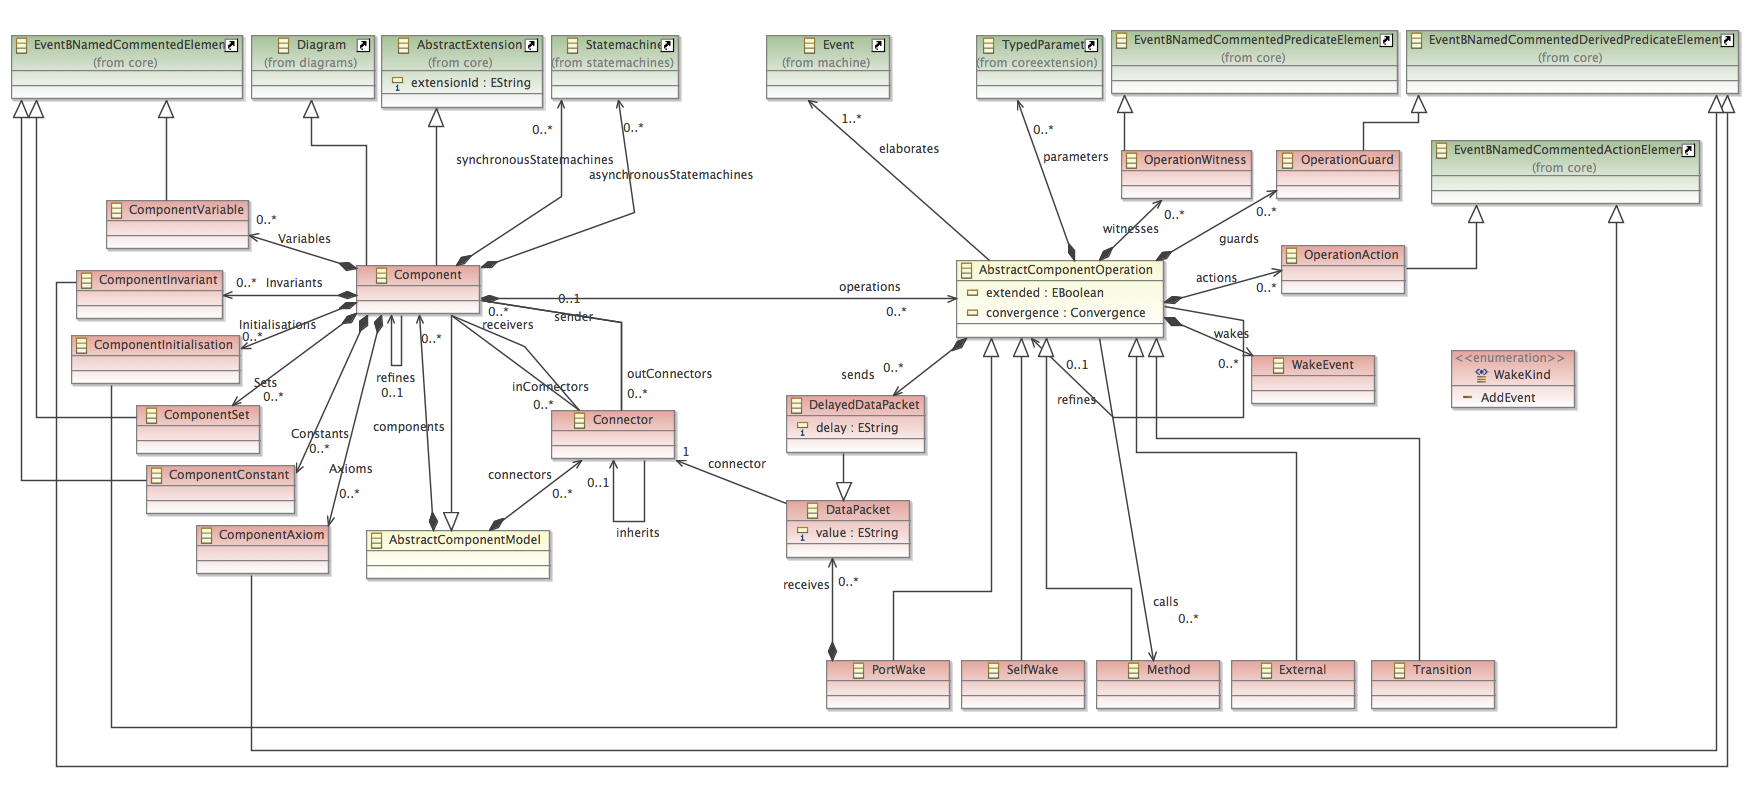
\includegraphics[width=1024]{figures/image1.png}
  \else
  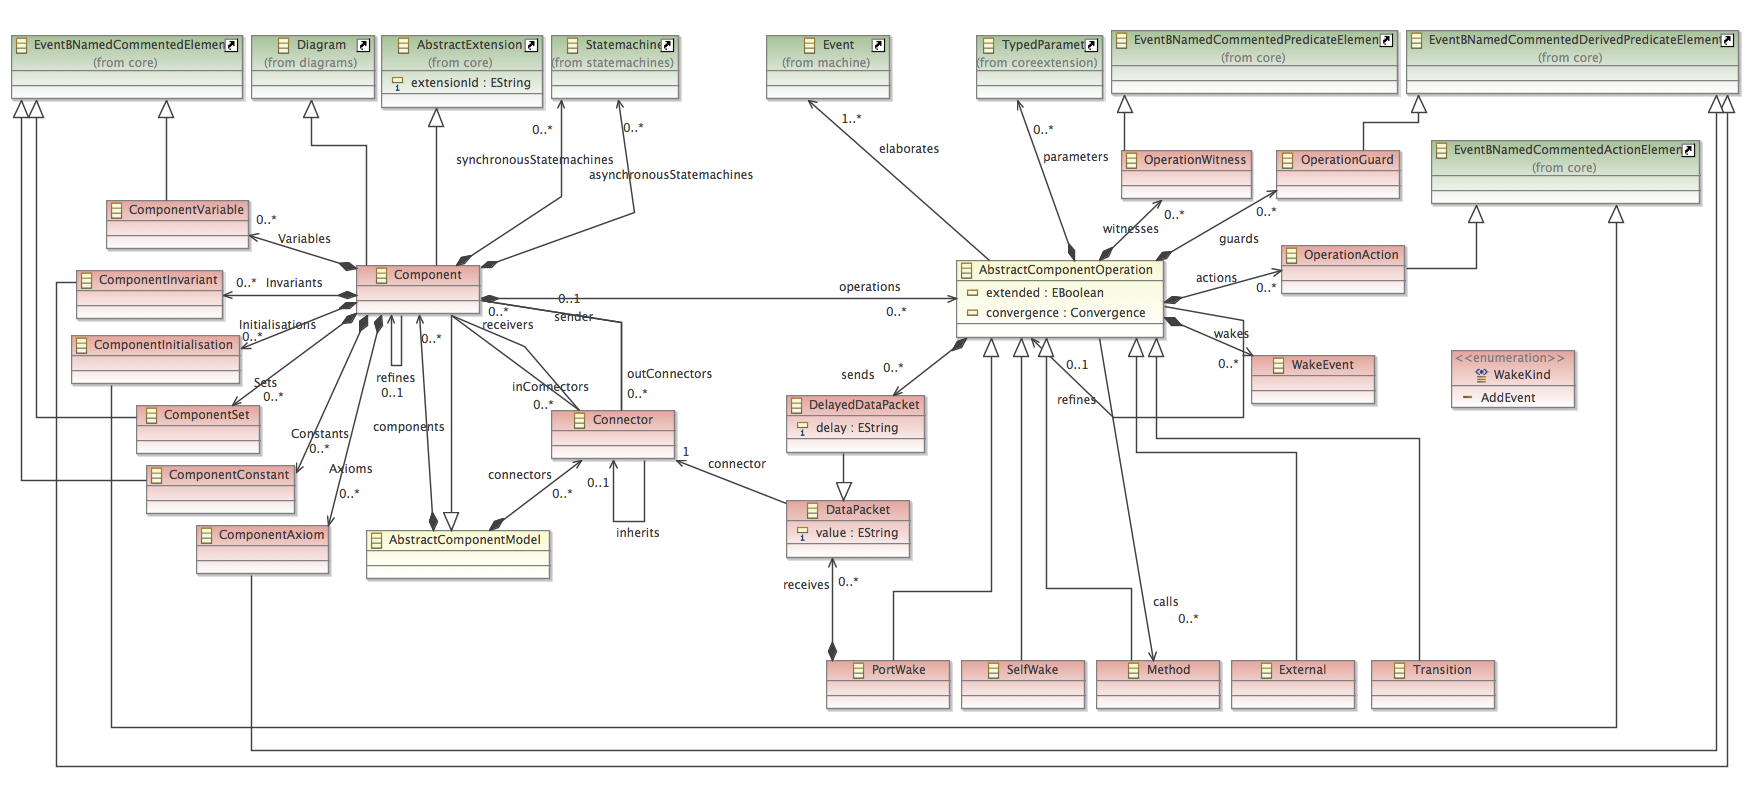
\includegraphics[width=1.0\textwidth]{figures/image1.png}
  \fi
  \caption{The CODA Meta-model}
  \label{fig:TheCodaMetamodel}
\end{figure}



The CODA Meta-model (Figure \ref{fig:TheCodaMetamodel}) defines an abstract syntax for the modelling language.
The boxes (called meta-classes) represent classes of elements that a particular CODA model might have.
In the diagram, the meta-classes are colour coded as follows.
Green indicates a referenced meta-class from another, more general, meta-model (i.e. not part of CODA), 
yellow indicates an abstract meta-class which can not be instantiated directly, but may be instantiated through one of its concrete specialised meta-classes and 
red indicates a concrete CODA meta-class that can be directly instantiated. 
These meta-classes are linked in three different kinds of ways:

\begin{itemize}
\item Generalisation indicates that instances of the source class are also instances of the target class. The targets properties are inherited by any meta-classes that specialise it.  For example, the meta-classes, \emph{PortWake}, \emph{SelfWake}, \emph{Method} etc. all specialise \emph{AbstractComponentOperation} so that operation properties such as \emph{sends} and \emph{wakes} do not have to be defined repeatedly. 
\item Containment indicates that instances of the source meta-class own instances of the target meta-class in a parent-child relationship. For example, any \emph{Component} may own a collection of\emph{AbstractComponentOperation}, which is referred to collectively as its \emph{operations}. 
\item Reference indicates that instances of the source meta-class may reference instances of the target meta-class. For example, any \emph{AbstractComponentOperation} may reference several\emph{Methods} via its \emph{calls} property although it does not contain them as children. 
\end{itemize}


%%% Local Variables:
%%% mode: latex
%%% TeX-master: "component_diagrams-user_manual"
%%% End:


\section{Running the Tool}
\label{sec:component_diagrams-running}

CODA is an extension of the Rodin Platform. See the Rodin User Handbook  for a full description of how to run the Rodin Platform and how to create and verify Event-B models.


Event-B models (including those with CODA models) can be imported and exported from the Rodin platform. Right-click anywhere in the Event-B Explorer view and select Import from the pop-up menu.
From the select window (Figure 2), select \textbf{\texttt{General - Existing Projects into Workspace}} and click on \textbf{\texttt{Next}}. (DO NOT select \textbf{\texttt{Archive File}}, even if you are about to import a zip file).
 


Figure 2 - Importing a Model Project


At the next window, select \textbf{\texttt{Select archive file}} and browse to your archived file. Any projects in the archive will be listed for selection in the centre pane of this window. (Make sure that \textbf{\texttt{copy projects into workspace}} is checked otherwise any changes will be made to the original copy). Click on \textbf{\texttt{Finish}}.


To export models, select the project(s) that you want to archive and choose \textbf{\texttt{Export}} from the pop-up menu. From the window that appears, select \textbf{\texttt{General-Archive File}} and press \textbf{\texttt{Next}}. Type in or browse to a location for the archive file and press \textbf{\texttt{Finish}} (Figure 3).
 

Figure 3 - Exporting a Model Project

%%% Local Variables:
%%% mode: latex
%%% TeX-master: "component_diagrams-user_manual"
%%% End:


\section{Building Models}
\label{sec:component_diagrams-buildingModels}

A CODA model is an Event-B model with component models as child elements of Event-B machines. Therefore, the first step is to create an Event-B project with an Event-B machine in it. To add a component model, right click on the Event-B machine and from the context menu (Figure \ref{fig:AddingaComponentModeltoaMachine}), select \textbf{\texttt{Add Component}}, and provide a name for the top-level component. Note that component models exist within components; therefore the top-level element is a single \emph{root} component which will contain the component model.
 

\begin{figure}[!htbp]
  \centering
  \ifplastex
  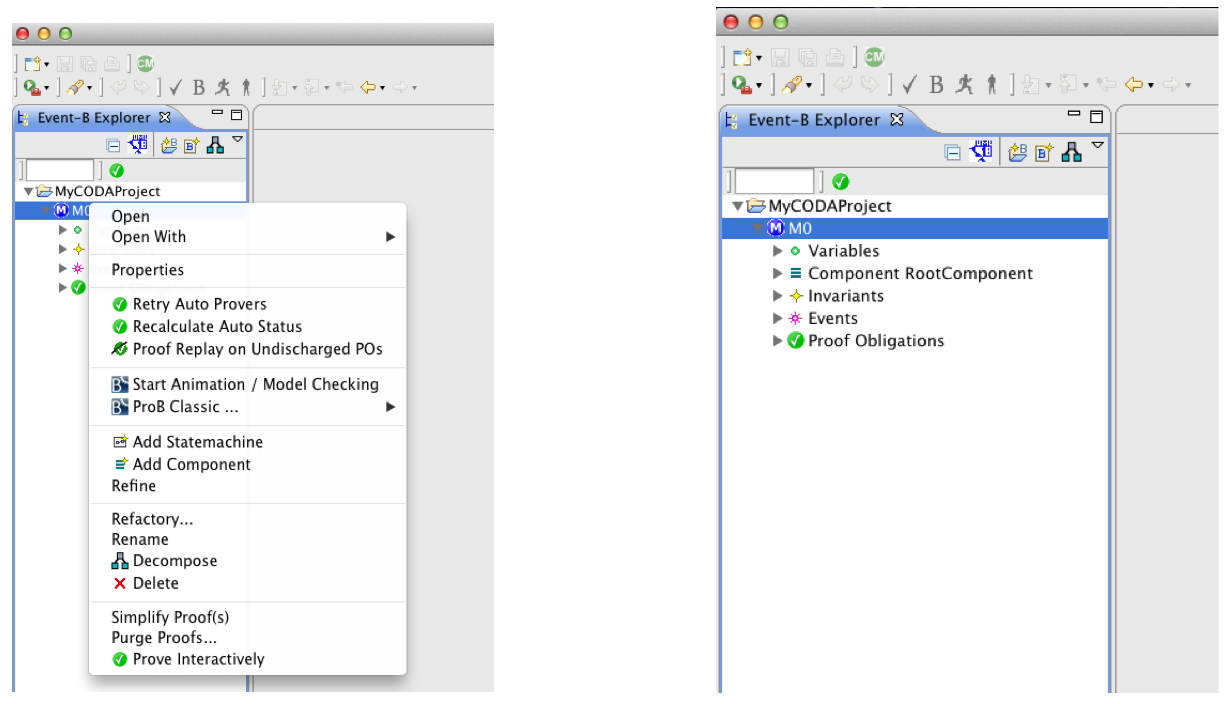
\includegraphics[width=768]{figures/image4.png}
  \else
  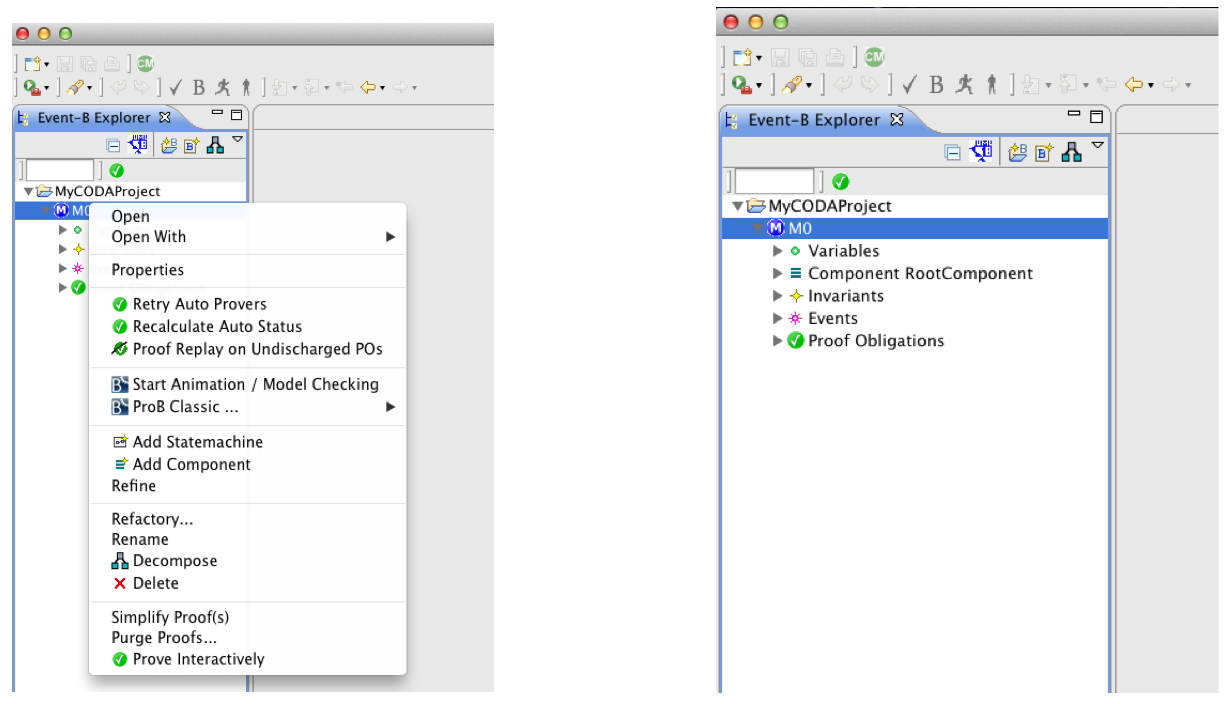
\includegraphics[width=0.75\textwidth]{figures/image4.png}
  \fi
  \caption{Adding a Component Model to a Machine}
  \label{fig:AddingaComponentModeltoaMachine}
\end{figure}


The component can now be opened for editing with the Component Diagram editor (Figure \ref{fig:TheComponentDiagramEditor}) by double clicking on it in the navigator tree.
 
\begin{figure}[!htbp]
  \centering
  \ifplastex
  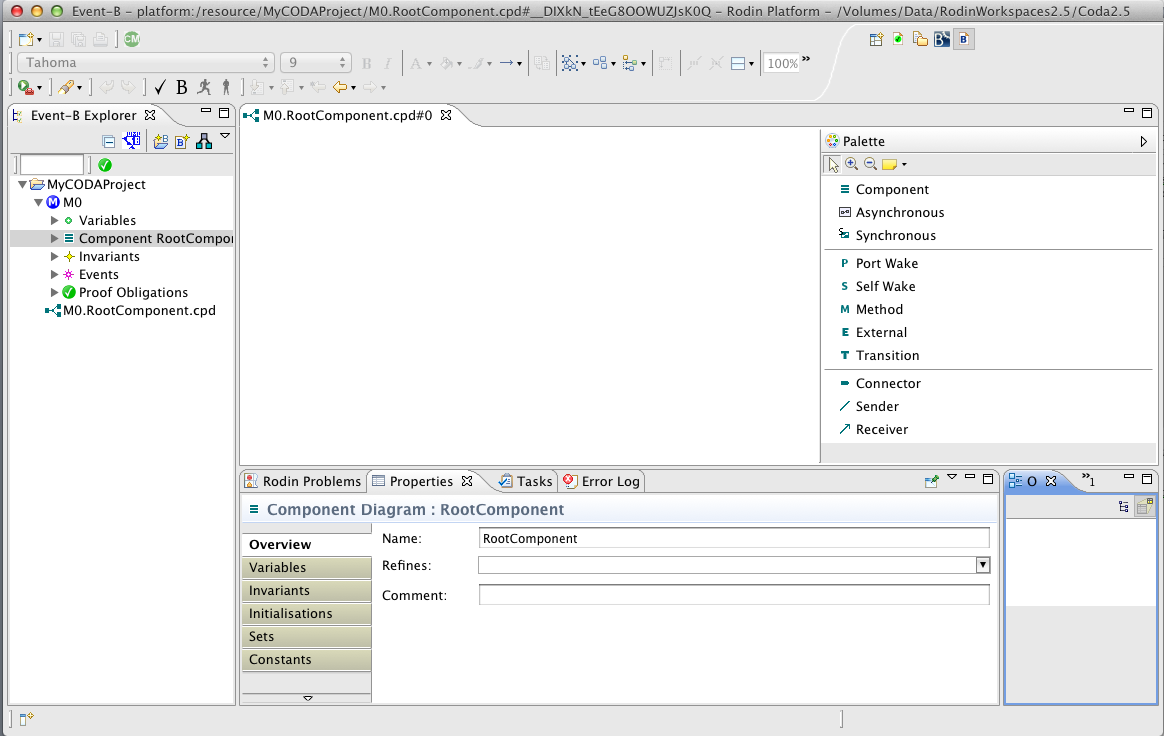
\includegraphics[width=1024]{figures/image5.png}
  \else
  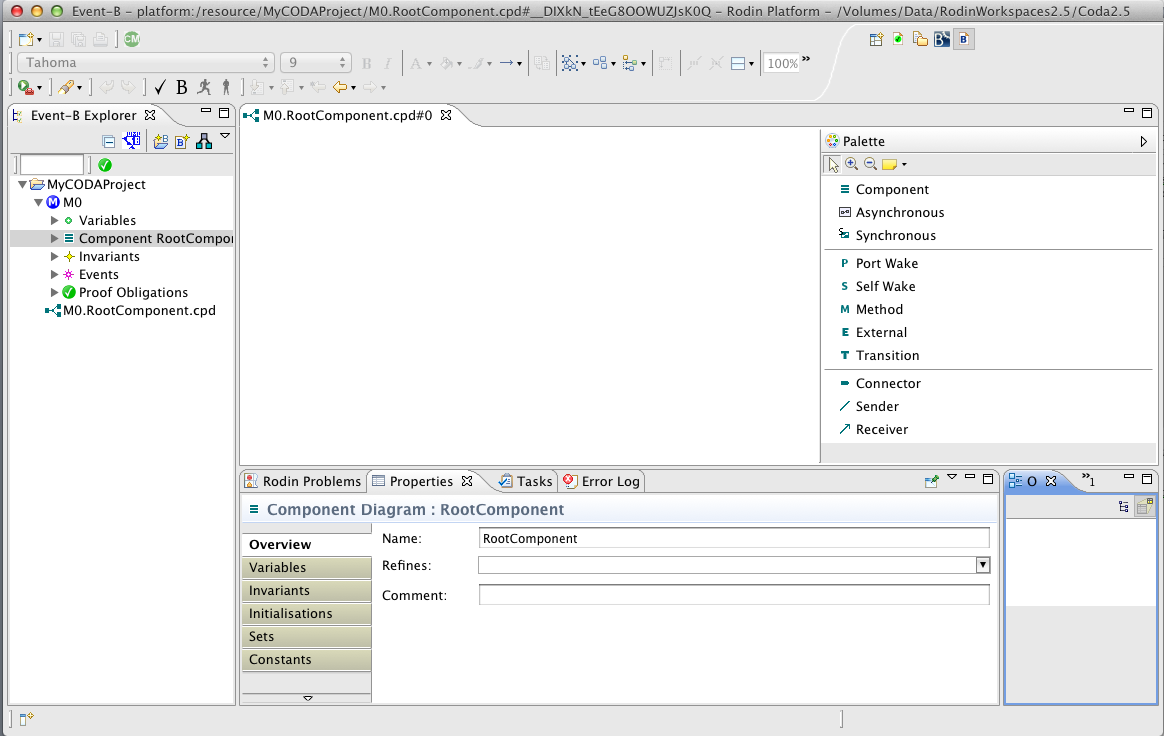
\includegraphics[width=1.0\textwidth]{figures/image5.png}
  \fi
  \caption{The Component Diagram Editor !!!TBD!!! THIS DIAGRAM SHOULD HAVE ANNOTATIONS - SEE WORD VERSION}
  \label{fig:TheComponentDiagramEditor}
\end{figure}


A component is created by clicking the Component item in the tool palette and then clicking on the canvas in the desired position for the component. (N.b. do not hold the mouse button on while doing this, just click and let go). Name the component either on the diagram or in the properties sheet name field.


A connector channel is created in a similar way. A link should be added to indicate which component sends on the connector. This is done by clicking on the Sender item in the tool palette and then click \& hold on the connector and dragging the link to the sending component. Similarly links can be added to indicate the receivers of the connector. (In both cases the link must be started from the connector and finished at a component).


Operations are added to a component by clicking on one of the tool palette operations and then clicking in the operations container of the parent component (Figure \ref{fig:Adding an Operation to a Component}). The different kinds of operation are briefly introduced in this section and illustrated in more detail in the tutorial section. Note that operations cannot be named because they derive their labels from the name of the events that they elaborate. The event elaboration property must be set in the properties editor using either the Add Event button (to link to an existing event) or the Create \& Add button to create a new event and link to it).


CODA models are based on Event-B and must be converted into equivalent Event-B models in order to perform verification. The Event-B generator is run by clicking the \textbf{B} icon in the toolbar menu (see Figure \ref{fig:TheComponentDiagramEditor}).


Event-B models consist of events that perform actions when their guards are true. CODA operations contribute guards and actions to an event that already exists in the underlying Event-B model. Operations may have ordinary guards and actions expressed in the Event-B notation but they may also have special kinds of guards and actions that are appropriate for the component modelling language. Furthermore, the operations themselves are specialised into several kinds for the component modelling language, which requires further guards and actions to be generated in the underlying Event-B. The following paragraphs introduce the specialised kinds of operations and the specialised kinds of guards and actions.
 
 \begin{figure}[!htbp]
  \centering
  \ifplastex
  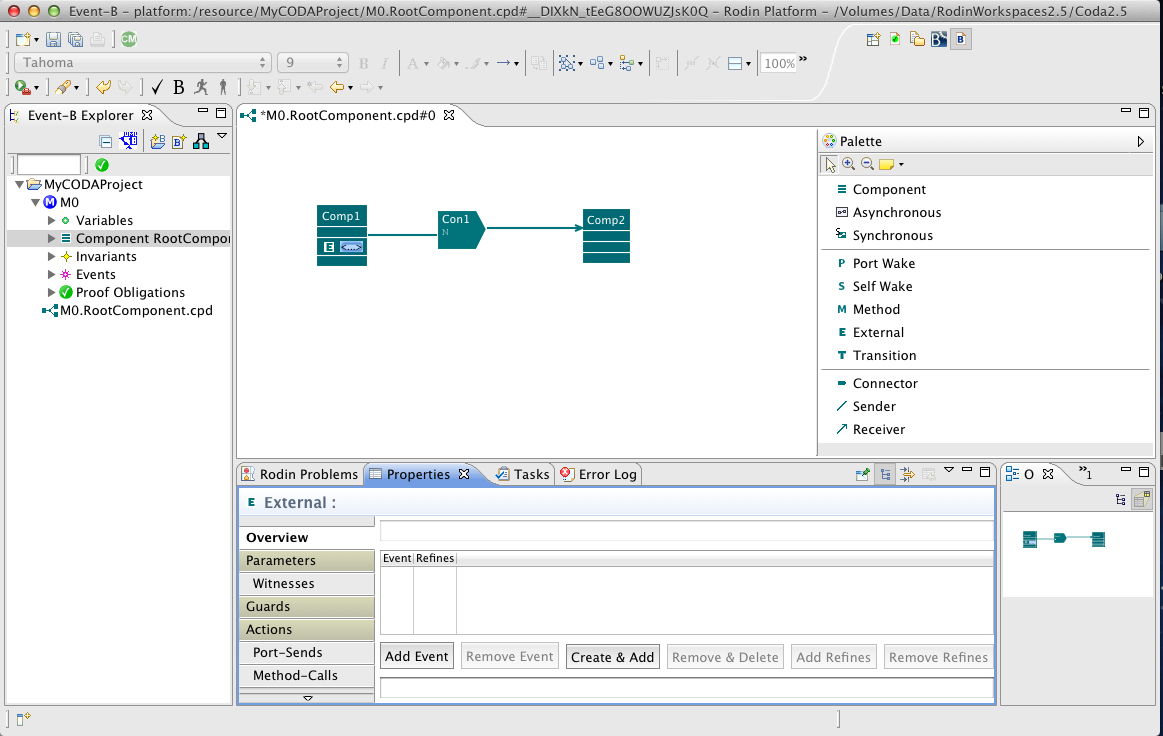
\includegraphics[width=768]{figures/image6.png}
  \else
  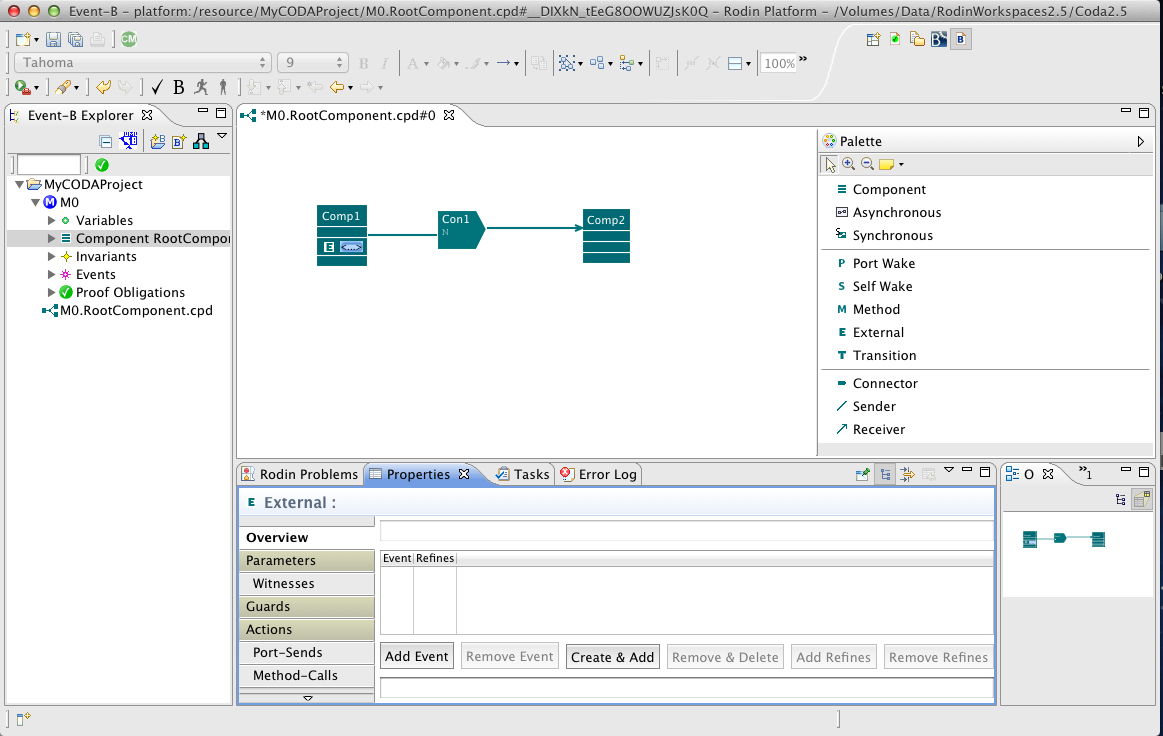
\includegraphics[width=0.75\textwidth]{figures/image6.png}
  \fi
  \caption{Adding an Operation to a Component}
  \label{fig:Adding an Operation to a Component}
\end{figure}


Having created operations they can be configured to send and receive on the connectors by adding port-send actions (Figure \ref{fig:AddingaSendActiontoanOperation}) and port-wake operations with port-wake guards. A port-send action represents the action of sending data over a connector and can be added to any operation in a component that has an outgoing connection to the connector. A port-wake operation is needed in the receiving component of the connector in order to respond to the receipt of data on the connector. These port-wake operations must have port-wake guards that define what connector data they respond to. 


\begin{figure}[!htbp]
  \centering
  \ifplastex
  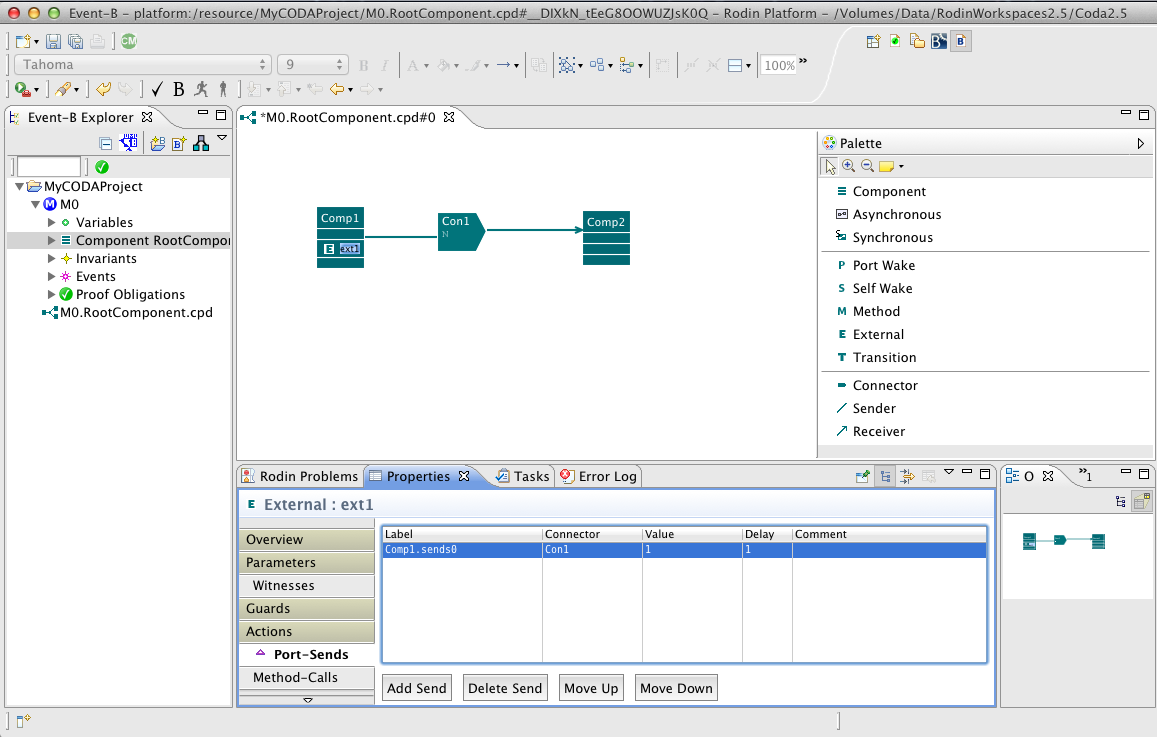
\includegraphics[width=768]{figures/image7.png}
  \else
  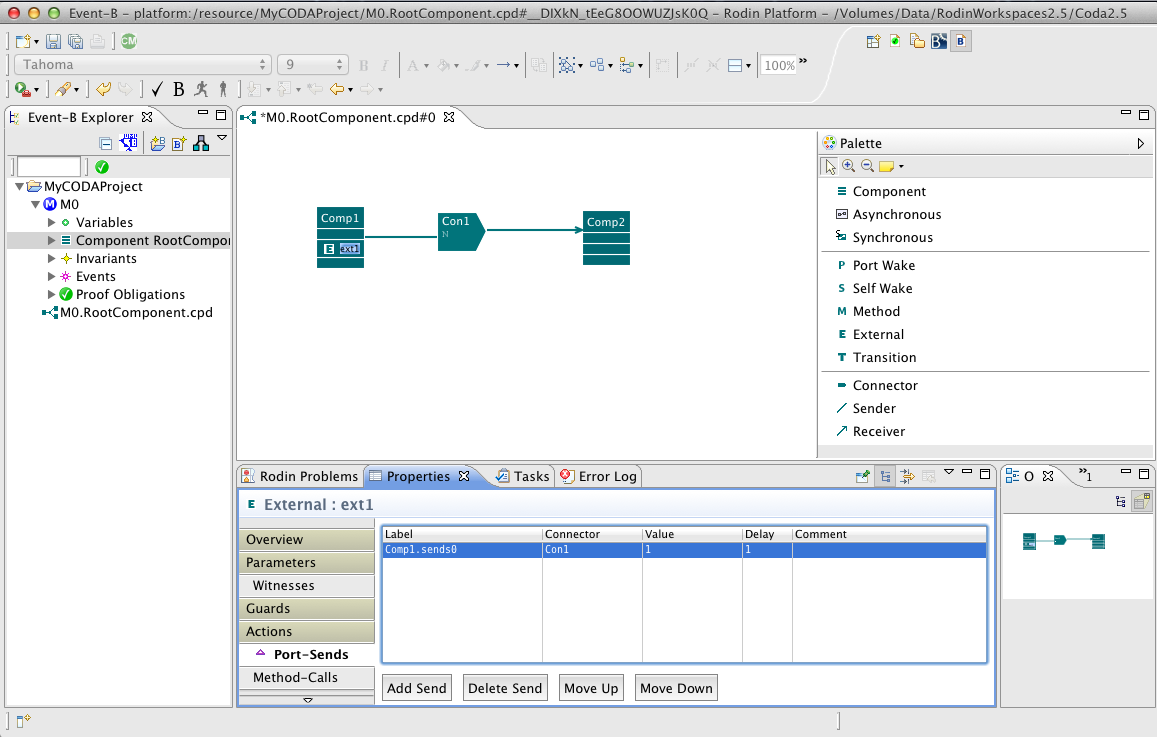
\includegraphics[width=0.75\textwidth]{figures/image7.png}
  \fi
  \caption{Adding a Send Action to an Operation}
  \label{fig:AddingaSendActiontoanOperation}
\end{figure}
 
 
Similarly, self-wake actions can be added to any operation and self-wake operations must be added to service them. A self-wake action represents the scheduling of a component wake-up at some future time and can be added to any operation in a component. A self-wake operation is needed in the component to respond to the component wake-up. 


Method call actions can be added to operations and method operations must be added to service the calls. A method call action immediately enables a particular method operation, which must then complete within the same clock cycle.


External operations represent events that occur in the environment that the model must respond to. The timing of these events is uncontrolled and therefore not synchronised to the clock in any way. These events may perform any of the operation actions (port-wake, self-wake, method calls) described here.


Data can be defined in the properties by selecting a component that represents the scope of the data (currently this scoping is not enforced). Note that the diagram canvas represents a root component and this may be the most appropriate place for global data. If any sets, constants or axioms are defined in this way an Event-B Context will be automatically generated to contain them.



State-machines may be added to components. Double clicking on the state-machine icon/name in the component opens a state-machine diagram. Since the state-machine diagram is a standard Rodin plugin (rather than part of the CODA specific tool) component behaviour such as port sends etc. cannot be added on the state-machine transitions. For this reason a special kind of component operation (Transition) is available in the component diagram. Transition operations must link to an event that is also linked to a state-machine transition. They enable component behaviour to be added to the components state-machine transitions. 


Two kinds of state-machine are available. Asynchronous state-machines are not linked to the clock whereas synchronous state-machines are tightly linked to the clock so that, while enabled, only one transition may be taken on each clock tick.




%%% Local Variables:
%%% mode: latex
%%% TeX-master: "component_diagrams-user_manual"
%%% End:


\section{Validation and Simulation}
\label{sec:component_diagrams-validation}

\subsection{Static Validation of diagram}
The static model validation checks that the model is well formed. The validation can be invoked at any time by clicking the V icon in the toolbar menu (see Figure 5). The validation is also invoked as a preliminary check when the generator is invoked. The validation rules fall into two categories; omissions that result in a meaningless model (reported as errors) and contraventions of the conventions of the components modelling notation that nevertheless can be translated to a meaningful Event-B model (reported as warnings). If the validation results in errors the generation does not proceed. If the validation raises warnings but no errors the generation proceeds. Note that model validation does not attempt to verify consistency properties of the model that will be checked by the Event-B static checker. The following validation rules are applied:

5.1.1	Errors

\begin{itemize}
\item The label of any labelled element (e.g. operations adopt a label from the events that they elaborate) shall not be null.
\item The name of any named element (e.g. Component, Connector) shall not be null.
\item The connector reference of a DataPacket (used in port sends and port wakes) shall not be null.
\item The value reference of a DataPacket shall not be null.
\item The delay value of a DelayedDataPacket (used in port sends) shall not be null.
\item The delay value of a WakeEvent shall not be null.
\item The wakeKind value of a WakeEvent shall not be null.
\item The type value of a Connector shall not be null.
\item The initial value of a Connector shall not be null.
\end{itemize}


5.1.2	Warnings

\begin{itemize}
\item An operation shall only send data to a connector that is an outgoing connector for the component that contains the operation
\item An operation shall only call methods that are contained in the component that contains the calling operation or in one of its sub-components.
\item A PortWake operation shall have at least one port wakeup.
\item A PortWake operation shall only receive port wakeups from a connector that is an incoming connector for the component that contains the PortWake operation.
\end{itemize}


\subsection{Model checking using ProB}
The ProB model checker can be used to verify the generated Event-B model. ProB is initiated by right clicking on a machine and then selecting Start Animation / Model Checking. The layout of the Rodin interface (perspective) should change to one similar to that shown in 
 

Figure 8 - ProB Model Checker Interface


The model can be animated by manually selecting enabled events from the view in the top left and observing the changes to the state in the centre view. However, it is recommended that the Oracle simulator is used for animation because it provides a higher-level interface oriented on the component model.
Model checking is invoked using the drop down menu from the checks toolbar item in the top-left Events view. The model checking options will then be displayed in a new window. Typical settings of these options are shown in Figure 9.

 
Figure 9 - ProB Model Checker Options


The generated model contains an infinite state space (due to the indefinite incrementing of time) and therefore the model checker will not complete its search of the state space. The model checker should be stopped manually after a short period and the coverage statistics can be examined to see the extent of coverage of the model. Since model checking does not complete it does not ensure that the model is consistent or deadlock free. However, the model checker often finds problems quickly and is therefore useful when trying to find problems in a model.
More details about running the ProB model checker are given here\footnote{\url{http://www.stups.uni-duesseldorf.de/ProB/index.php5/User_Manual}}.


\subsection{State-machine Animation}


State-machines may be animated by clicking the running man icon in the toolbar menu (see Figure 5). The currently active state (if any) is shown with a bold outline. Any enabled transitions (i.e. transitions that are linked to at least one event that is enabled) are shown in green and the event may be selected for execution by clicking on the transition and selecting from the pop-up list. The state-machine animation is a view to the Pro-B model checker and during animation, all of the Pro-B interface is also available. Usually the state-machine will only represent part of the model and it will be necessary to fire some events from the ProB Events view when no transitions are enabled. State-machine animation provides a clearer view of the behaviour of the state-machine part of the model so that its interaction with other variables and events of the model can be validated. State-machine animation is not essential but may be a useful optional validation step.
 

Figure 10 - State-machine Animation Interface
The animation can be terminated by clicking the stood man icon in the toolbar menu (see Figure 5).


\subsection{Simulation of Component model}
The CODA simulator is based on ProB but provides an interface that is aware of the CODA components model. The interface consists of an additional view that is presented as part of the ProB perspective (the lower view in Figure 11). The simulator is started by right clicking on a machine and selecting Simulation-Start. 
 

Figure 11 - CODA Simulator User Interface


5.4.1	Modes

During simulation there are two modes. Recording, where a new gold run is being recorded or playback where a previous gold run is being replayed for comparison. During recording the user controls which operations execute whereas during playback the system controls which operations execute. 

5.4.2	Recording Mode

During recording mode, operations can be invoked manually from the enabled operations table or via one of the three left hand buttons on the control panel. These buttons have the following functions. Tick N selects operations non-deterministically from those that are enabled until the clock has advanced by the number of clock ticks configured in the adjacent panel. Step selects one operation non-deterministically from those that are enabled. Continue, selects operations non-deterministically from those that are enabled until a choice between two operations of the same component is required. To ensure the latter button terminates a limit (20) of the number of operations is applied. 
At any point the gold run can be saved by pressing the Save button or discarded by pressing the Restart or Replay buttons. The Restart button remains in record mode and the Replay button switches to playback mode.

5.4.3	Playback Mode

During playback mode, a previous gold run is selected and its operations are replayed. Operations may not be selected from the enabled operations table. The three buttons in the control panel have slightly different behaviour. Tick N selects operations from the sequence defined in the gold run until the clock has advanced by the number of clock ticks configured in the adjacent panel. Step selects the next operation from the gold run. Continue, selects operations from the gold run until it is exhausted or the limit (20) of the number of operations is reached.
At any point the playback run can be saved by pressing the Save button or discarded by pressing the Restart button. The Restart button remains in playback mode. At any time (whether saved or not) the playback can be left and continued in record mode by pressing the Stop button. This enables a previous gold recording to be extended or a different branch to be taken at any point.

5.4.4	Summary of Control Buttons
\begin{itemize}
\item 
\item Save - [recording | playback] Saves the current trace model and continues in the same mode. (The trace model is a gold run when in recording mode and a normal run in playback mode.
\item Stop - [playback] Leaves playback and continues in recording mode. (The trace from playback is continued so that it can be extended to make a new gold run). When in recording mode, does nothing.
\item Restart - [recording | playback] Discards the current trace and re-starts animation in the same mode as before. (In playback mode, the same gold run is replayed).
\item Replay - [recording] Leaves recording mode and enters playback mode. The current trace is discarded and reset. A gold run for playback is chosen and loaded via a user dialog.
\end{itemize}

 
Figure 12 - Model of CODA Simulator Operation

5.4.5	Saved Trace runs

The gold and playback runs are saved into a folder, called Oracle in the project that is being simulated. The file names for the runs are auto generated using the following scheme.

Gold runs:
<Machine name>.test.<timestamp>.gold.oracle 

Playback runs:
<Machine name>.test.<timestamp>.oracle 


%%% Local Variables:
%%% mode: latex
%%% TeX-master: "component_diagrams-user_manual"
%%% End:


\section{Tutorial}
\label{sec:component_diagrams-tutorial}

This section illustrates the use of the CODA modelling tool and a proposed methodology via an example model development. The tutorial shows how to construct models using the tool, how to add detail through refinement, and how to verify and validate the models using the ProB model-checker and the CODA Simulator. The models are also verified by proof but interactive proof (when proof obligations are not discharge automatically) is beyond the scope of this tutorial.
 
 \subsection{The Top-level Abstract Model}
\label{sec:component_diagrams-tutorial_topLevelAbstractModel}


The modelling process begins by describing a single, abstract state machine that represents the washing machine together with its environment. Four states represent the modes of the system: IDLE, WASHING, RINSING and SPINNING and seven transitions represent how the system modes evolve. A component WM is also introduced to represent the complete system. It contains the state-machine and owns operations that link to the transitions in the state-machine. The top-level component and state machine are shown in Figure \ref{fig:AbstractModelOfAWashingMachine}.
At this stage the transition operations in the component WM add little to the model but they are needed due to a limitation (explained below) of the representation of self-wake events. Since self-wake events are modelled in Event-B by a single generated variable per component, any operations of a component that, in future refinements, alter the state of self-wakes must be added when the component is first introduced. If they were added later the rules of refinement would prevent them from altering the self-wake variable.

 \begin{figure}[!htbp]
  \centering
  \ifplastex
  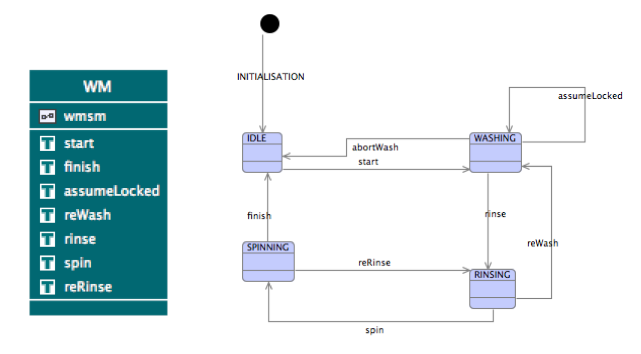
\includegraphics[width=1024]{figures/image13.png}
  \else
  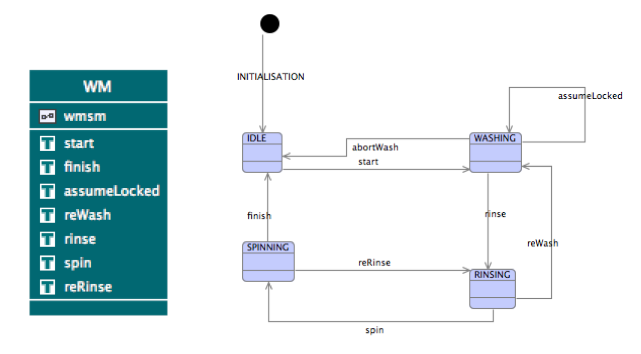
\includegraphics[width=1\textwidth]{figures/image13.png}
  \fi
  \caption{Abstract Model of a Washing Machine}
  \label{fig:AbstractModelOfAWashingMachine}
\end{figure} 

This system-level state machine is untimed and non-deterministic. For instance, when the system is in state RINSING, the system will immediately move to either state SPINNING or WASHING non-deterministically. The state machine represents all the possible mode traces of the system.
Once the state machine has been constructed, the first step is to ensure that all the proof obligations that have been generated by the CODA tool are discharged successfully, as shown in Figure \ref{fig:DischargedProofObligationsOfTheAbstractModel} below. Usually, if the user has added no extra invariants to the model, all the proof obligations should be discharged automatically. If any proof obligations have not been discharged (indicated by an orange question mark icon) they should be examined to determine whether there is a problem with the model. To examine a proof obligation, double click on its icon in the navigator. Switch to the proving perspective by clicking the green tick icon in the right hand corner of the menu bar.  Examine the goal as well as the information tab to work out what the prover is attempting to prove.
 
 \begin{figure}[!htbp]
  \centering
  \ifplastex
  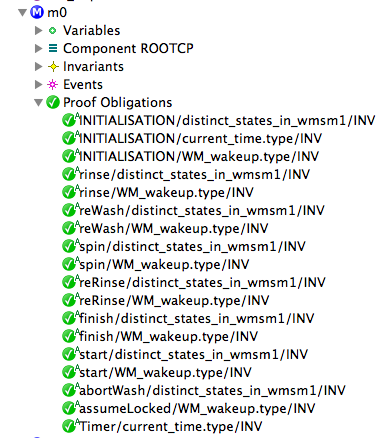
\includegraphics[width=1024]{figures/image14.png}
  \else
  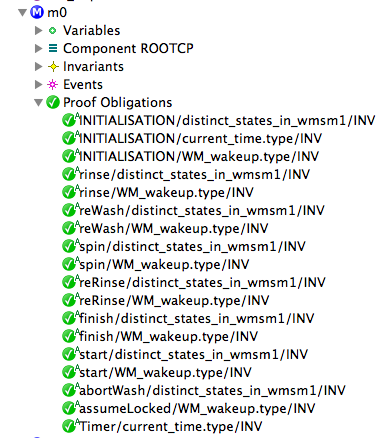
\includegraphics[width=1\textwidth]{figures/image14.png}
  \fi
  \caption{Discharged Proof Obligations of the Abstract Model}
  \label{fig:DischargedProofObligationsOfTheAbstractModel}
\end{figure} 

The next step in the process is to animate the system-level state machine to validate that states and transitions correctly represent the system-level view of the washing machine as shown in Figure \ref{fig:AnimatingTheStatemachineOfTheAbstractModel}. This is a validation process requiring subjective evaluation of the model against system requirements. Does the state-machine behave as desired?

 \begin{figure}[!htbp]
  \centering
  \ifplastex
  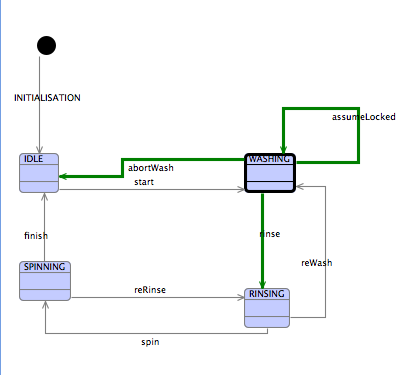
\includegraphics[width=1024]{figures/image15.png}
  \else
  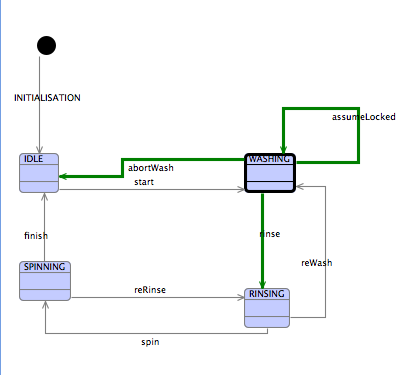
\includegraphics[width=1\textwidth]{figures/image15.png}
  \fi
  \caption{Animating the State-machine of the Abstract Model}
  \label{fig:AnimatingTheStatemachineOfTheAbstractModel}
\end{figure} 

The current state of the system is WASHING, as indicated by the bold, black outline of the state. Three transitions, highlighted in green, are enabled from this state: abortWash, rinse and assumeLocked. Select one from this non-deterministic choice to proceed with the animation. Continue animating the state machine to validate this top-level specification against the system requirements.
The specification may also be validated from the ProB view of Rodin as shown in Figure \ref{fig:AnimatingTheAbstractModelWithProBEventAndHistoryViews} and Figure \ref{fig:AnimatingTheAbstractModelWithProBStateView} below. The event view of Figure  \ref{fig:AnimatingTheAbstractModelWithProBEventAndHistoryViews} presents a list of enabled events from which one may be selected to advance the animation. The history view of Figure  \ref{fig:AnimatingTheAbstractModelWithProBEventAndHistoryViews} shows a record of previous selections. At any stage of the animation it is possible to go back to a selection in the history and perform a new animation from that point.
 
 \begin{figure}[!htbp]
  \centering
  \ifplastex
  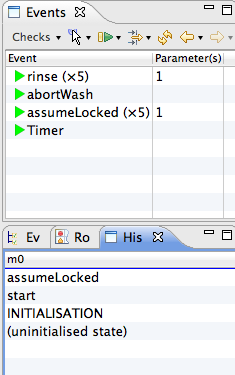
\includegraphics[width=1024]{figures/image16.png}
  \else
  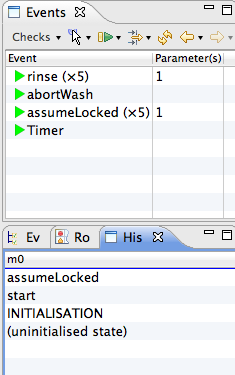
\includegraphics[width=1\textwidth]{figures/image16.png}
  \fi
  \caption{Animating the Abstract Model with ProB Event and History Views}
  \label{fig:AnimatingTheAbstractModelWithProBEventAndHistoryViews}
\end{figure} 

The state view of Figure \ref{fig:AnimatingTheAbstractModelWithProBStateView} shows the current and previous value for each variable. The invariants and guards may also be analysed in this view. The final verification step is to show absence of deadlock using the ProB model checker.

 \begin{figure}[!htbp]
  \centering
  \ifplastex
  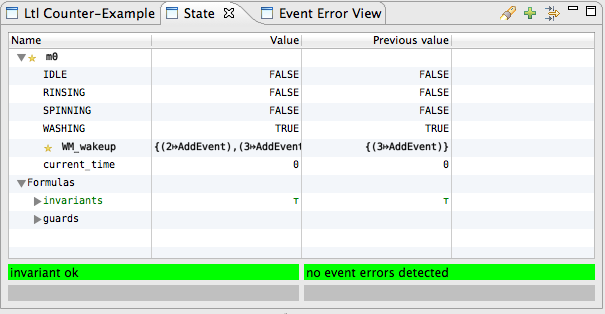
\includegraphics[width=1024]{figures/image17.png}
  \else
  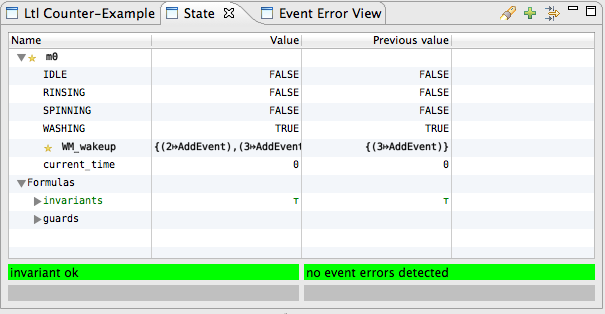
\includegraphics[width=1\textwidth]{figures/image17.png}
  \fi
  \caption{Animating the Abstract Model with ProB State View}
  \label{fig:AnimatingTheAbstractModelWithProBStateView}
\end{figure} 

First the model checker is configured as shown in Figure \ref{fig:ProBModelCheckerOptions} to find deadlocks and invariant violations. For this abstract model, the automatic provers have already proved all the proof obligations, but later in the refinement process it may be more difficult to prove some of the invariants. The model checker can then be used to look for counterexamples that are due to modelling errors. If the model checker reveals a counterexample it is more efficient than embarking on a complex proof that is eventually found to be false. If a counterexample is not revealed (and the complete state space has not been covered) the goal of the proof may still be false. Therefore the goals to be proven should be examined carefully as they often reveal a problem with the model. 
It is important not to leave unproven invariants in a model since if they are not true these could be used in later refinements by the automatic provers to make incorrect deductions.
Selecting symmetry reduction option is not really necessary at this stage, but can help to reduce model checking time when the model is more complex.
When the model checking completes, the results are presented by ProB in the window shown in Figure \ref{fig:ProBModelCheckingCoverageForTheAbstractModel} below.
 
 \begin{figure}[!htbp]
  \centering
  \ifplastex
  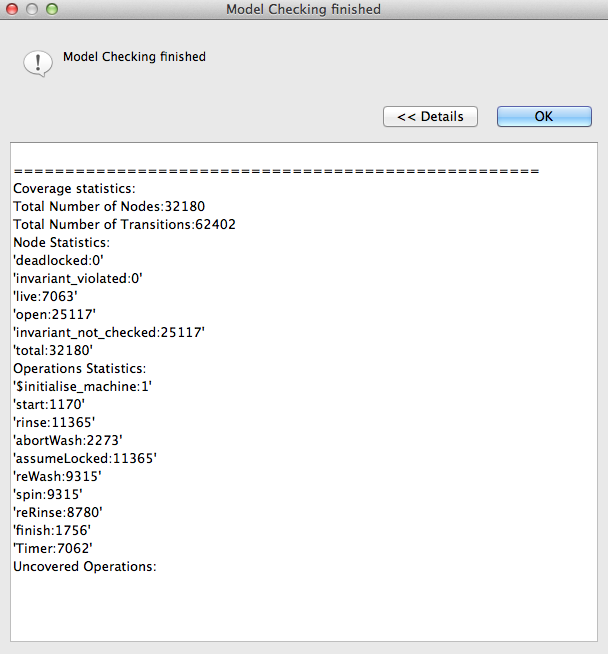
\includegraphics[width=1024]{figures/image18.png}
  \else
  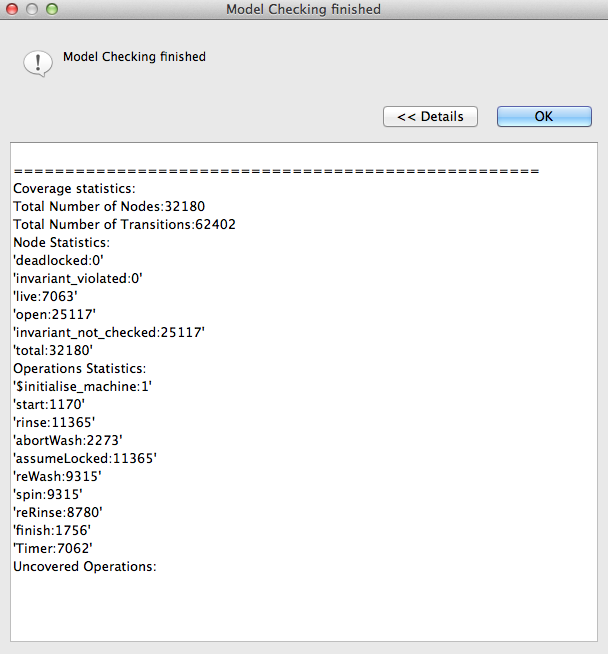
\includegraphics[width=1\textwidth]{figures/image18.png}
  \fi
  \caption{ProB Model Checking Coverage for the Abstract Model}
  \label{fig:ProBModelCheckingCoverageForTheAbstractModel}
\end{figure} 

The interesting coverage metric is shown at the bottom of the window: Uncovered Operations. In this case all operations have been covered which increases confidence in the absence of deadlock.

%%% Local Variables:
%%% mode: latex
%%% TeX-master: "component_diagrams-user_manual"
%%% End:

 \subsection{The First Refinement}
\label{sec:component_diagrams-tutorial_firstRefinement}


The single component and abstract state machine is now refined into a system comprising two components as shown in Figure 20 below. The first component is the Control Panel and the second the abstract washing machine sub-system. Two connectors enable communication between the two components. The first connector, CI, is used to pass the Washing Program ID (PID) to the washing machine sub-system and the second connector, WMSTATE, passes the status of the sub-system back to the Control Panel to be displayed. The state machine is unchanged except for the addition of a self transition on state IDLE which constrains the sendWaiting operation so that it only sends the waiting status over the WMSTATE connector while the washing machine is idle.
 
Figure 20 - First Refinement of Washing Machine

The external operation, UserStart, in component CP represents the user starting the wash by passing the selected wash program, using a port-send action on connector CI to the washing machine sub-system. The port-send action is shown in Figure 21. Note that the minimum delay of 1 is used. The value pid1 is a parameter representing the non-deterministic sending of any PID.
 
Figure 21 - First Refinement : Port Sends on CI

A corresponding port-wake operation, start, in the washing machine sub-system receives the program ID that will, in a subsequent refinement, be decoded to control the wash. The port-wake guard is shown in Figure 22. 
A further port-wake operation, ignoreStart, manages inadvertent start requests from the user. Note that this is necessary due to a design decision not to constrain the sending of start messages from CP. If WM is not in a state to respond to the start an explicit ignoreStart is needed to avoid the system deadlocking.
 
Figure 22 - First Refinement : Port Wakes on CI

When the washing machine sub-system receives the pid, it responds with a port-send action on connector WMSTATE to inform the Control Panel that the washing machine is now RUNNING as shown in Figure 23
 
Figure 23 - First Refinement : Port Sends on WMSTATE

The Control Panel receives the message from the washing machine sub-system with the port-wake operation Running shown in Figure 24 so that this information can be displayed to the washing machine user.
 
Figure 24 - First Refinement : Port Wakes on WMSTATE

The State Machine Animation facility is now used again to validate this 2-component system and the model checker is run to check for deadlocks as shown in Figure 25. Note that, again, all operations have been covered by the model checker.
 
Figure 25 - ProB Model Checking Coverage for the First Refinement


%%% Local Variables:
%%% mode: latex
%%% TeX-master: "component_diagrams-user_manual"
%%% End:

 \subsection{The Second Refinement}
\label{sec:component_diagrams-tutorial_secondRefinement}


The washing machine sub-system component is now further refined, as shown in Figure 26, into two components, the DOOR sub-system and an abstract component, WM, that represents the rest of the washing machine sub-system. Two connectors enable communication between these two components. The first, lock, passes a Boolean signal to the DOOR sub-system to lock the door. The second, doorPosition, informs the Washing Machine sub-system when the door is opened or closed.
 
Figure 26 - Second Refinement of Washing Machine

Note that the DOOR component has two external operations, closeDoor and openDoor, which represent the interaction of the user with the door. Care is needed in this refinement to ensure that the system cannot get into an unsafe state; the door should always be locked when the washing machine is washing, rinsing or spinning so that the user cannot inadvertently open the door and release potentially very hot water.
The state-machine for the washing machine is refined to split the WASHING state into sub-states LOCKINGDOOR and INPROGRESS and IDLE into UNLOCKINGDOOR and IDLEWAITING, Figure 27. This is necessary to accommodate the new transitions concerned with locking and unlocking the door.
 
Figure 27 - Second Refinement : Refined State-machine of the Washing Machine

An invariant, DOORLOCKED  = TRUE, is introduced in the sub-system state machine for states INPROGRESS, RINSING and SPINNING.
The state machine for the door sub-system is shown in Figure 28. The door may be open (DOOROPEN) in which case any instructions to lock the door are ignored (ignoreLock) or it may be closed (DOORCLOSED). When the door is closed it may be unlocked (DOORUNLOCKED) or locked (DOORLOCKED). Note that the transitions unlockDoor and lockDoor are drawn with the superstate DOORCLOSED as their source indicating that they can fire irrespective of whether the door is locked or not.
 
Figure 28 - Second Refinement : State-machine for the Door Component

The washing machine sub-system sends a message via the lock connector to the door sub-system to lock the door if it has received a message from the door via the doorPosition connector indicating that the door is closed.  The washing machine sub-system then initiates a self-wake, delayed by 3 time units, as shown in Figure 29. If the door is still closed at the self-wake, as indicated by the guard 
WM\_doorPosition = CLOSED,  then it is assumed that the door is locked and the system can proceed to the INPROGRESS state. The alternative transition (Figure 27) is abortWash which has the negated guard  WM\_doorPosition $\neq$ CLOSED.
 
Figure 29 - Second Refinement : Self Wake to Check Door Locked

The proof obligations generated for the safety invariant are difficult to discharge. It is a good idea at this stage to proceed immediately to animation and model checking, to ensure that the model behaves as expected.
Model checking does indeed show immediately that the safety invariant is violated and provides a counterexample in the history pane as shown in Figure 30.
 
Figure 30 - Counterexample Discovered by ProB

Although the refinement models the latency that certainly exists between the washing machine sub-system and door sub-system, it allows the user to open and close the door repeatedly in zero-time. Modelling this Zeno Behaviour is unrealistic and results in a scenario where the user can close the door and then open it again immediately just before it is locked.
The solution is to model more realistically the latency that must exist in the opening and closing of the door by introducing a delay on the External Event, closeDoor, as shown in Figure 31. The guard  \textbf{\code{current\_time > DOOR\_latency}}, where DOOR\_latency is a variable that is set to current\_time + 1 by any preceding door open or close events, ensures that two door events cannot occur on consecutive clock ticks. This corresponds to an assumption that the systems time response makes it impossible to open and close the door without it being detected. This is sufficient to ensure that any changes of door state are successfully transmitted to the WM component.
 
Figure 31 - Introducing Latency to the Door Operations
 
The model checker is re-run to verify that the invariant violation has been addressed and that there is no deadlock, as shown in Figure 32. Note now, that the model checking results show that not all operations have been covered, though examination of the guards and actions of these uncovered operations show that none are material to the invariant violation being investigated. Although not a proof, model checking with operation coverage gives confidence that the model is behaving as expected.
 
Figure 32 - ProB Model Checking Coverage for the Second Refinement 
 
To improve operation coverage, it is a good idea to try the alternative Breadth First Search option. Figure 33 shows the improved coverage results and Figure 34 shows how this option is set.
 
Figure 33 - ProB Model Checking Coverage for the Second Refinement : Breadth First
 
Figure 34 - Configuration for ProB Model Checker Breadth First Option
 
%%% Local Variables:
%%% mode: latex
%%% TeX-master: "component_diagrams-user_manual"
%%% End:

 \subsection{The Third Refinement}
\label{sec:component_diagrams-tutorial_thirdRefinement}
 
Now we refine the notion of the Program. We associate with each PID a washTime, rinseTime and spinTime and also introduce a WashCount and SpinCount as shown in Figure 35. These properties constrain and make deterministic the operation of the washing machine sub-system for a given PID.
 
Figure 35 - Adding Wash Program Details to the Model
 
The delay introduced for each wash mode is modelled using a SelfWake as shown for the rinse mode in Figure 36.
 
Figure 36 - Introducing Wash Program Delays using Self Wakes
 
The number of washes or rinses associated with a program is modelled using a counter which is decremented and hence completes at rinseCounter = 0, as shown in Figure 37.
 
Figure 37 - Introducing Wash Program Cycles using Guards
 
Again, the model checker is run to verify that no deadlocks have been introduced into the system. Since this refinement is only to strengthen the guards, invariant preservation is not an issue in this refinement. Note that as shown in Figure 38, full operation coverage is achieved. The program constraints introduced in this refinement have reduced the model state space. 
 
Figure 38 - ProB Model Checking Coverage for the Third Refinement
 
The state machine is shown in Figure 39 below. Invariants concerning the counters have been added to the INPROGRESS and RINSING states. These invariants help ensure that no mistakes have been made in constructing the counters.
 
Figure 39 - State-machine for the Third Refinement 
 

%%% Local Variables:
%%% mode: latex
%%% TeX-master: "component_diagrams-user_manual"
%%% End:

 \subsection{The Fourth Refinement}
\label{sec:component_diagrams-tutorial_fourthRefinement}

 
The washing machine sub-system is now further partitioned into 2 components: the drum sub-system and an abstract component representing the remaining washing machine sub-system, following the pattern of previous refinements.
The component diagram is shown in Figure \ref{fig:FourthRefinementOfWashingMachine}.
Three boolean connectors pass messages from the washing machine sub-system to the drum to open and close the hot or cold water valves and to switch the drain pump on or off. Two further natural number connectors pass the water level and the water temperature back from the drum to the washing machine sub-system.
 
 \begin{figure}[!htbp]
  \centering
  \ifplastex
  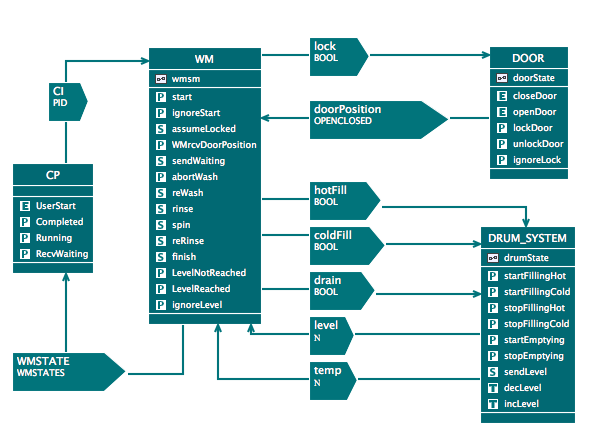
\includegraphics[width=1024]{figures/image41.png}
  \else
  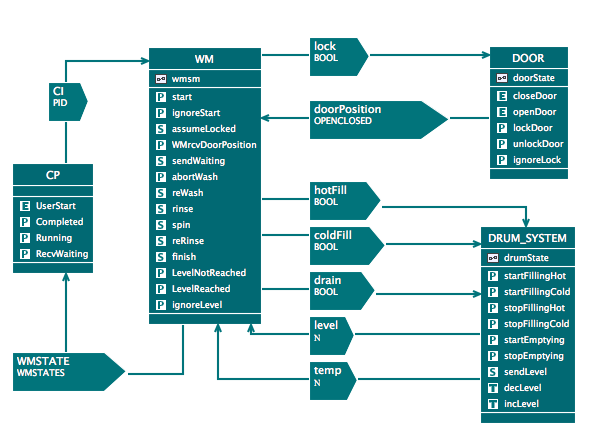
\includegraphics[width=1\textwidth]{figures/image41.png}
  \fi
  \caption{Fourth Refinement of Washing Machine}
  \label{fig:FourthRefinementOfWashingMachine}
\end{figure} 
 
The state machine for the drum sub-system is shown in Figure \ref{fig:FourthRefinementStatemachineForTheDrumComponent}.
 
 \begin{figure}[!htbp]
  \centering
  \ifplastex
  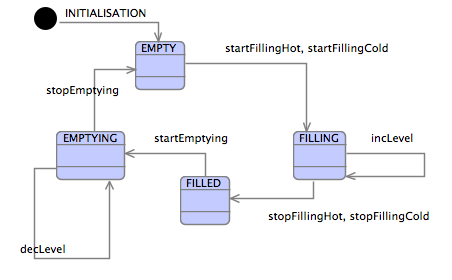
\includegraphics[width=1024]{figures/image42.png}
  \else
  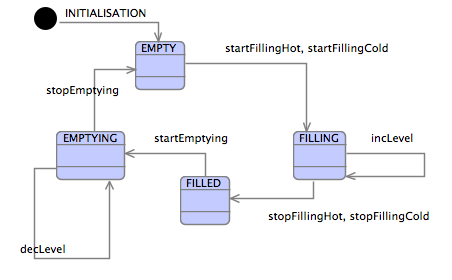
\includegraphics[width=1\textwidth]{figures/image42.png}
  \fi
  \caption{Fourth Refinement : State-machine for the Drum Component}
  \label{fig:FourthRefinementStatemachineForTheDrumComponent}
\end{figure} 
 
The washing machine state machine is now further refined to manage the filling and emptying of the drum by monitoring the water level as shown in Figure \ref{fig:FourthRefinementRefinedStatemachineOfTheWashingMachine}.
 
 \begin{figure}[!htbp]
  \centering
  \ifplastex
  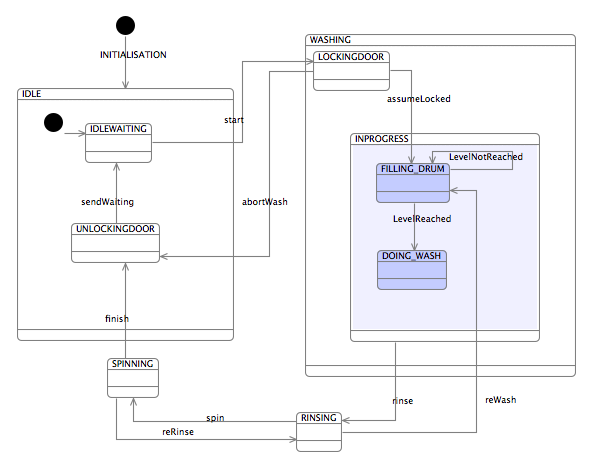
\includegraphics[width=1024]{figures/image43.png}
  \else
  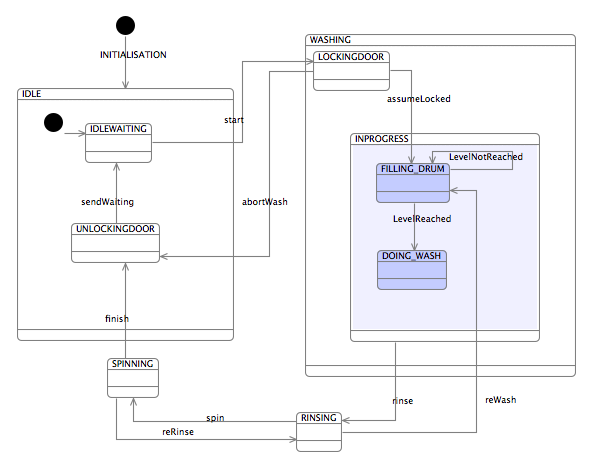
\includegraphics[width=1\textwidth]{figures/image43.png}
  \fi
  \caption{Fourth Refinement : Refined State-machine of the Washing Machine}
  \label{fig:FourthRefinementRefinedStatemachineOfTheWashingMachine}
\end{figure}  
 
The value TRUE is sent on the coldFill connector as shown in Figure \ref{fig:FourthRefinementPortSendOnTheColdFillConnector}.
 
 \begin{figure}[!htbp]
  \centering
  \ifplastex
  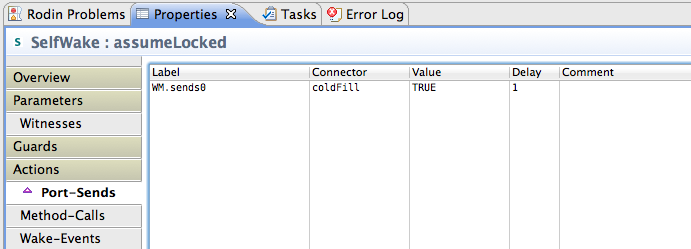
\includegraphics[width=1024]{figures/image44.png}
  \else
  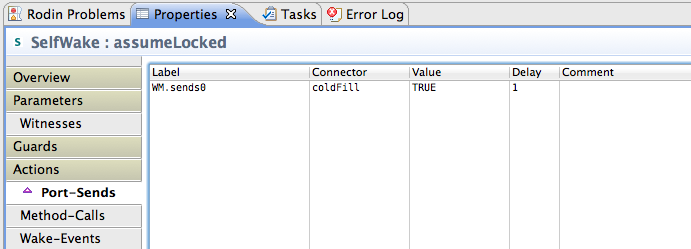
\includegraphics[width=1\textwidth]{figures/image44.png}
  \fi
  \caption{Fourth Refinement : Port Send on the coldFill Connector}
  \label{fig:FourthRefinementPortSendOnTheColdFillConnector}
\end{figure} 
 
The drum sub-system receives the value on the coldFill connector and starts filling the drum (Figure \ref{fig:FourthRefinementPortWakeOnTheColdFillConnector}).
 
 \begin{figure}[!htbp]
  \centering
  \ifplastex
  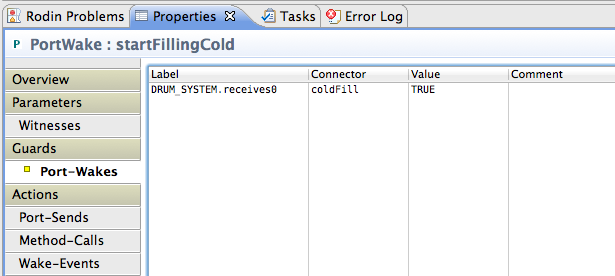
\includegraphics[width=1024]{figures/image45.png}
  \else
  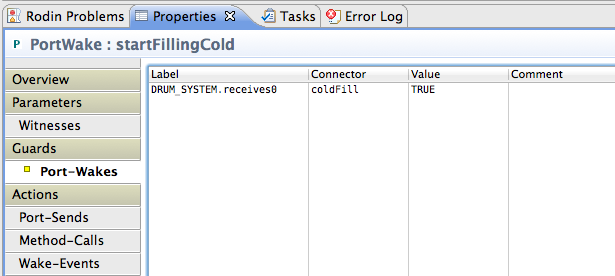
\includegraphics[width=1\textwidth]{figures/image45.png}
  \fi
  \caption{Fourth Refinement : Port Wake on the coldFill Connector}
  \label{fig:FourthRefinementPortWakeOnTheColdFillConnector}
\end{figure}  
 
The drum sub-system sends the value of water level and water temperature repeatedly at unit delay intervals using the self-wake operation sendLevel of Figure \ref{fig:FourthRefinementSelfWakeToRepeatedlySendOnLevelAndTempConnectors}.
 
 \begin{figure}[!htbp]
  \centering
  \ifplastex
  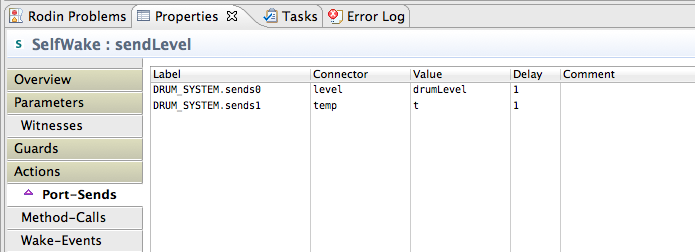
\includegraphics[width=1024]{figures/image46.png}
  \else
  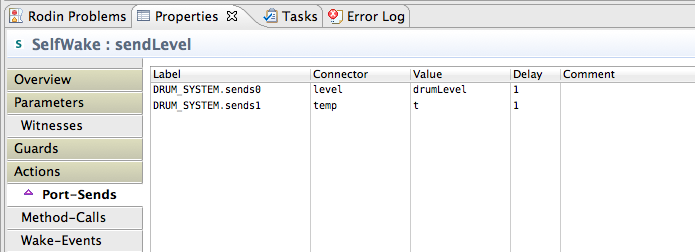
\includegraphics[width=1\textwidth]{figures/image46.png}
  \fi
  \caption{Fourth Refinement : Self Wake to Repeatedly Send on level and temp Connectors}
  \label{fig:FourthRefinementSelfWakeToRepeatedlySendOnLevelAndTempConnectors}
\end{figure} 
 
The washing machine sub-system switches off the water valve when it detects that the water level associated with the PID has been reached, as shown in Figure \ref{fig:FourthRefinementGuardedPortWakeToRespondWhenLevelReached}.
 
 \begin{figure}[!htbp]
  \centering
  \ifplastex
  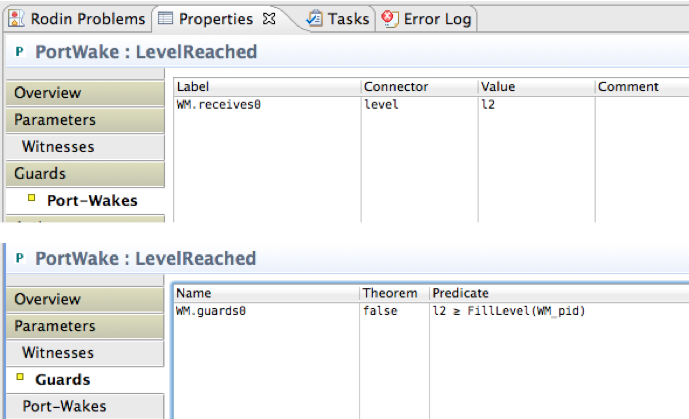
\includegraphics[width=1024]{figures/image47.png}
  \else
  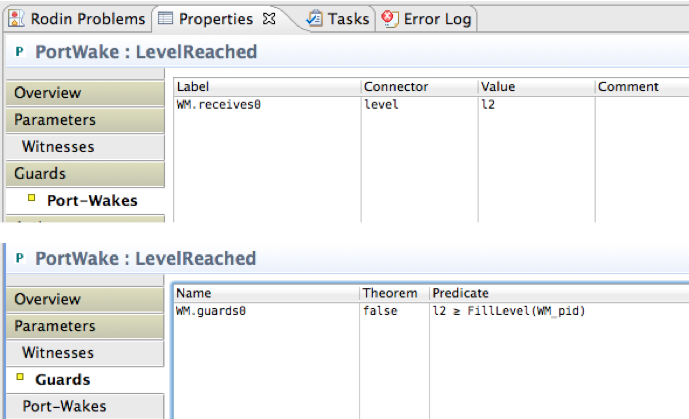
\includegraphics[width=1\textwidth]{figures/image47.png}
  \fi
  \caption{Fourth Refinement : Guarded Port Wake to Respond when Level Reached}
  \label{fig:FourthRefinementGuardedPortWakeToRespondWhenLevelReached}
\end{figure}  
 
The model checker is run again to show absence of deadlock. Note that because of the added complexity of this refinement, not all operations are covered (Figure \ref{fig:ProBModelCheckingCoverageForTheFourthRefinement}). Sufficient operations, however, have been covered to give confidence that filling operation is performing satisfactorily.
 
 \begin{figure}[!htbp]
  \centering
  \ifplastex
  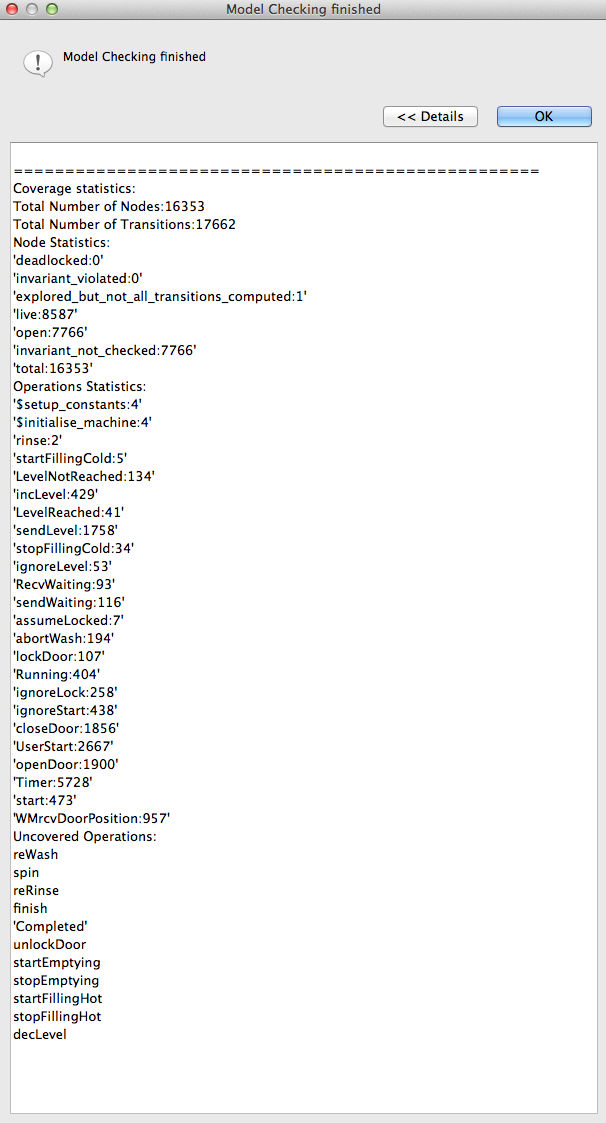
\includegraphics[width=1024]{figures/image48.png}
  \else
  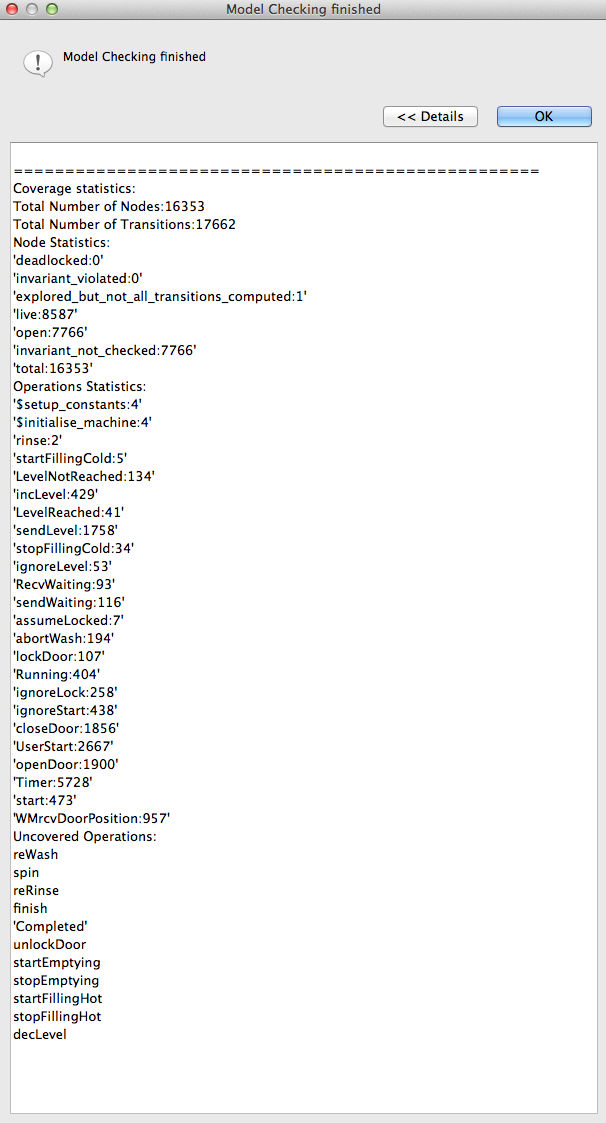
\includegraphics[width=1\textwidth]{figures/image48.png}
  \fi
  \caption{ProB Model Checking Coverage for the Fourth Refinement}
  \label{fig:ProBModelCheckingCoverageForTheFourthRefinement}
\end{figure}  


%%% Local Variables:
%%% mode: latex
%%% TeX-master: "component_diagrams-user_manual"
%%% End:

 
\subsection{Further Refinements}
 
The refinement strategy that has been established in the earlier refinements can continue as the agitator motor and heater components are introduced. At each stage the abstract washing machine sub-system component is constrained until it finally represents just the
  hardware/software controller
   that is being developed for the washing machine.
 
\subsection{Running the Oracle Simulator}
 
The CODA simulator can be used at every refinement step to establish a set of regression tests and golden results. Figure 48 illustrates the state of the system at times 10, 14, 15 and 18.

Figure 48 - Snapshots of CODA Simulator at Times 10, 14, 15 and 18
 
\subsection{Conclusion}
 
A method for system modelling and refinement has been illustrated using the washing machine case study example. Modelling begins with an abstract state machine model of the system, which is systematically refined into a set of communicating processes - the hardware/software controller under development and the components that represent the controller environment.
At each refinement step, formal proof and model checking is used to validate the model against the requirements and to show absence of deadlock.
The final hardware/software controller component can then be verified within a component-based environment using the CODA Oracle Simulator.

%%% Local Variables:
%%% mode: latex
%%% TeX-master: "component_diagrams-user_manual"
%%% End:


\section{I/O level Refinement}
\label{sec:component_diagrams-ioLevel}

The tutorial in the previous section demonstrates how to perform abstract modelling and refinement using the CODA component diagram tools. This section illustrates how a refinement can be introduced which models the hardware I/O level behaviour. The model uses a synchronised state-machine, which allows a sequence of clock synchronised I/O events to be performed in order to achieve an abstract data transmission.


Figure 49 - Abstract Model of a Controller Sending an Enable Message to a Device 

In the abstract model, shown in Figure 49, a Controller component sends data to enable a Device component. This is modelled as a port-send belonging to a self-wake operation SendData, a connector chan and a port-wake operation Enable. The self-wake is scheduled by the RecvPowerUp operation, so that its timing represents the completion of an envisaged concrete operation which takes time to complete.

Figure 50 - Refined Model : Controller Sending a Bit Level Signal to a Device

In the refined model, shown in Figure 50, the concrete data transmission operations are introduced. In this example, two connectors are used, A for the data bit stream and B for a data ready semaphore. Operations, SetA, SetB, ResetA and ResetB send 1 and 0 on these connector channels respectively. In order to ensure these operations are invoked in the desired iterative sequence, a synchronised state-machine IO is attached to the Controller component. 

Figure 51 - Refined Model : I/O Level State-machine

The transitions of this state-machine, Figure 51, are linked to the same events as the component operations that send the data bits. Hence these operations are constrained to execute in the iterative sequence defined by the state-machine. Furthermore, because this is a synchronised state-machine, it is forced to fire exactly one transition on each clock cycle while it is enabled. The state-machine becomes enabled when the initial transition is taken and this is linked to a method operation of the Controller component that is called by the RecvPowerUp operation. Guards and Actions in the bit sending operations allow the state-machine to complete 16 cyclic sequences before taking the FinishIO transition that disables the state-machine. The data sent by the operation SendData was calculated to be received by operation Enable at the same clock cycle as the last bit is received on connector A representing the end of the bit level transmission.
In this refinement the abstract data connector and associated operation behaviour have been retained although they are now redundant because they are replaced by the I/O level connector behaviour. It would be tempting to remove the abstract data connector and prove that the I/O level is a refinement of it. However, it may be useful to retain the abstract data connector for later generation of temporal assertions in generated output such as VHDL.

%%% Local Variables:
%%% mode: latex
%%% TeX-master: "component_diagrams-user_manual"
%%% End:


\section{Refactoring}
\label{sec:component_diagrams-refactoring}

A refactoring facility is provided in iUML-B that allows a set of changes made to the collection of iUML-B diagrams in an abstract model to be propagated down the refinement chain as part of a commit action. Alternatively, the set of changes can be reverted, restoring the model to its pre-change state.
Changes cannot be committed (hence propagated) when a lower refinement also has uncommitted changes. I.e. if several refinements have uncommitted changes they must be committed or reverted in order starting from the most refined level and working up the refinement chain. 
Changes are only propagated to a refinement when they are still relevant to the refinement. Changes may have already been made in the refinement, as part of the refinement process, that mean that a subsequent change in the abstract model cannot be propagated. For example the parent element of a changed attribute may have been removed and replaced with a different model element or a guards predicate may have been edited to utilise new variables introduced in the refinement. Changes to Event-B formula attributes (i.e. predicates and actions) are only propagated when the equivalent refined formula is unchanged except for formatting (whitespace).

\subsection{Enabling Refactoring}

The refactoring facility may be enabled or disabled in the iUML-B preferences menu. The current default is DISABLED.  
WARNING: If this preference is disabled while there are outstanding, uncommitted changes, and the associated model is then edited without refactoring being enabled, those change records will become invalid and wont be able to be propagated at a later stage.

Figure 55 - Preference for enabling refactoring.

\subsection{Automatic Archiving}

An archive of the complete project including any change records and reports is made before a commit is attempted. This is in case an unexpected event such as power failure should cause the commit to fail leaving the model in a corrupted state. In this case the project should be deleted and restored from the archive using the standard Eclipse import facility (\textbf{\texttt{Import - General - Existing Projects into Workspace - Select archive file}}).

\subsection{Decorator}

Machines with outstanding, uncommitted changes are decorated in the Event-B Explorer. 

Figure 56 - Decorator indicating outstanding recorded changes (see M0).

\subsection{Refactoring Menu: Commit and Revert}

The Commit and Revert actions are accessed from a pop-up context menu, by right clicking on a machine that has outstanding uncommitted changes.

Figure 57 - Context menu for Commit/Revert.

\textbf{Commit} -
When Commit is selected for a machine that has outstanding uncommitted changes, firstly an information and confirmation message appears. This gives the user a chance to cancel since the Commit operation is a significant process that can only be reversed by restoring from archive.

Figure 58 - Commit confirmation message.

If ok is selected on Mi, the following steps will be taken
\begin{enumerate}
\item any open diagrams will be closed, 
\item the project will be archived,
\item the recorded changes for Mi will be propagated to the next level refinement Mi+1 (if any),
\item the changes made to the refinement Mi+1 will be recorded,
\item the previous change records for Mi will be deleted,
\item all diagrams of the previous model Mi will be generated,
\item steps 3 to 6 will be repeated for the refinement Mi+1,
\item a report of the complete process will be saved.
\end{enumerate}


\textbf{Revert} -
When Revert is selected for a machine that has outstanding uncommitted changes, firstly an information message appears. This gives the user a chance to cancel since the Revert operation is a significant process that cannot be reversed.

Figure 59 - Revert confirmation message.

If ok is selected on a machine Mi, the following steps will be taken
\begin{enumerate}
\item any open diagrams will be closed,
\item the changes made to Mi will be reverted taking the model back to its original state,
\item the change records for Mi will be deleted,
\item all diagrams of Mi will be generated.
\end{enumerate}


\textbf{No Changes} - 
If Commit or Revert are selected for a machine that has no recorded changes, an appropriate message is displayed and no further action is taken.

Figure 60 - No changes error message.


\subsection{Resources: Change Records and Reporting}

Various resources are created to support refactoring. In normal use it is not necessary to access these resources and they are not visible in the Event-B Explorer by default. If it is wished to examine the generated reports or the change records they can be viewed either by opening a standard eclipse workspace file navigator or Project Explorer (using Window-Show View) or by un-selecting the All files and folders filter of the Event-B Explorer. (The second method is shown here).

Figure 61 - Removing \texttt{All files and folders} filter for Event-B Explorer.

The various resources that are generated are as follows. 
As soon as a supported editor is opened two files will appear in a folder called /iumlb/changes/ within the project. These are:
$<$myMachine$>$\_bum.xmb  -  a copy of the pre-change state of the model,
$<$myMachine$>$\_bum.equivmap - a map from the elements in the xmb file to the corresponding elements in the Rodin  model. 
These files can be opened for examination but if they are edited the refactoring process is likely to fail. The xmb file can be opened with an EMF editor such as Rose. The equivmap file can be opened with a normal text editor.
As soon as some changes to the diagram are saved a change record will appear in the same folder, $<$myMachine$>$\_bum.changes.  Again, the file can be opened with an EMF editor such as Rose but any alterations are likely to cause the refactoring process to fail.

Figure 62 - Changes resources produced for refactoring.

Note: If these three files are deleted the project will be left in its current state with no record of changes. This can be useful if for some reason it is wished to neither commit nor revert the changes but to leave the models as they are with the abstract model edited but the changes not propagated. 
If the changes are reverted, once the revert process has completed, these three files are deleted.
If the changes are committed, once the commit has completed, these three files are deleted and a file $<$myMachine$>$\_bum.$<$timestamp$>$.report is created in the folder /iumlb/reports/. This is a text file giving a detailed record of the changes made down the refinement chain.

Figure 63 - Reports produced by refactoring

%%% Local Variables:
%%% mode: latex
%%% TeX-master: "component_diagrams-user_manual"
%%% End:


\section{Translation to Event-B}
\label{sec:component_diagrams-translation}



Key:
\begin{itemize}
\item Transition Identifier
\item Wake Queue Identifier
\item Connector Identifier
\item Connector Type
\item Connector Value
\item Time Interval (NAT)
\end{itemize}


\subsection{Current time}

A variable current\_time models the progression of time slices.  Generated once per model.
 
\begin{table}[htbp]
\centering
\begin{tabular}{|l|l|l|}
\hline
SOURCE & \multicolumn{2}{l|}{GENERATED} \\ \hline
\multirow{3}{*}{For each root component model} & VARIABLE & current\_time \\ \cline{2-3} 
 & INVARIANT & current\_time $\in$ NAT\\ \cline{2-3} 
 & INITIALISATION & current\_time = 0 \\ \hline
\end{tabular}
\caption{Translation of root components to current\_time variables}
\label{transaltion-CurrentTime}
\end{table}
 
If there is more than one root component model in a machine, the root component name will be used as a prefix for each current\_time variable.

\subsection{Connector}
 
A Connector is a special kind of a variable with a different translation. 
 
TODO: TABLE TO GO HERE

 \subsection{Component Wake-up}

A component can be scheduled to wake at some time interval in the future by adding to a queue of wake events. The wake may occur non-deterministically within a specified time interval . A component may have a number of different wake queues for different purposes and to allow new wake-ups to be added in refinements. Each wake queue generates two extra variables to contain the schedule event times for enabling the wake events and disabling the timer. This is implemented so as to allow for different kinds of wake event, for example, a collection of interrupt priorities. At the moment only one kind (AddEvent) will be used. A further kind (NullEvent) is reserved for null queue entries, such as the initial one queued at initialisation (which is there to avoid well-definedness problems with max. These entries have no effect. A synchronisation variable is also generated for each wake queue to provide a way to synchronise the wake events with the timer. It is a set containing the min times of all wake events that have been serviced.
 
 TODO: TABLE TO GO HERE
 

%
\subsection{Synchronisation of Operations}


\subsubsection{External and Transition Operations}

An External operation is a special kind of operation that represents a response to some external trigger event (e.g. a button press). 
A Transition operation must be linked to an event that is also linked to by a transition in a state-machine that is contained in the same component.
Both External and Transition operations are un-synchronised with the clock. They shall not be triggered by connectors and are not scheduled by self-wakes. They may read and write to connectors and call other methods and may schedule component wake events.

\subsubsection{Port-Wake Operations}

For synchronisation, port-wake operations are grouped according to the combination of incoming connectors that they respond to. Therefore if two port-wake operations in the same component have port-wake properties on the same group of connectors they will use the same synchronisation flag and hence exactly one of them will respond to the simultaneous arrival of data on that group of connectors.  Which one does so may be controlled via other guards such as particular values arriving on the connectors.

TODO: TABLE TO GO HERE


Port-wake operations are synchronised using these flags.

TODO: TABLE TO GO HERE


Port-wake operations are triggered by values arriving on connectors.

TODO: TABLE TO GO HERE


\subsubsection{Self-Wake Operations}

When a component wake up event is reached, all of the components self-wake operations that are waiting on that wake queue are enabled subject to their other guards. This enablement remains even if the current\_time is further increased. They are also guarded by (and set) the wake queues synchronisation variable to ensure that exactly one self-wake operation responds to the wake event. The synchronisation variable contains the min times of all the wake events from that queue that have been processed. If the latest (i.e. maximum) min time is not in the synchronisation variable, the event is enabled. (Note that the timer is not prevented from progressing until the max time for the wake event is reached).

TODO: TABLE TO GO HERE

\subsubsection{Method Operations}

A method is a special kind of synchronised operation that is called directly from another operation. Methods shall not be triggered by connectors and shall not be re-scheduled by self-wakes. Methods may read and write to connectors and call other methods. 

TODO: TABLE TO GO HERE

\subsection{Actions by Operations}

Every operation (both synchronised and un-synchronised) may call method operations.

TODO: TABLE TO GO HERE

Every operation (both synchronised and un-synchronised) may send to connectors.

TODO: TABLE TO GO HERE


Every operation (both synchronised and un-synchronised) may set wake events.

TODO: TABLE TO GO HERE

\subsection{Synchronised State-machines}

Synchronised state machines are synchronised with the timer so that while they are enabled, exactly one transition is taken per clock tick. The state-machine becomes enabled when its initial transition is taken and becomes disabled when its final transition is taken. The following is in addition to the normal state machine generation, which is not part of CODA.
Enable and synchronisation flags are generated for each synchronised state-machine.

TODO: TABLE TO GO HERE

For each transition in a synchronised statemachine, the flags are used as follows:

TODO: TABLE TO GO HERE


\subsection{Process Statemachines}

Process state machines represent a sequence of steps (forming a process) which, once enabled, runs and completes within a single timer tick. The state-machine becomes enabled when its initial transition is taken and becomes disabled when its final transition is taken. While the statemachine is enabled the timer is disabled. The following is in addition to the normal state machine generation, which is not part of CODA. The initial transition should be linked to component operations to control when the process is initiated.
An enable flag is generated for each process state-machine. 

TODO: TABLE TO GO HERE

For each transition in a process statemachine, the flags are used as follows:

TODO: TABLE TO GO HERE

\subsection{Timer}

A special event is generated to advance time when the current time slice has completed.

TODO: TABLE TO GO HERE

		



%%% Local Variables:
%%% mode: latex
%%% TeX-master: "component_diagrams-user_manual"
%%% End:



%\section{Getting Started}
\label{sec:component_diagrams-getting-started}






%%% Local Variables:
%%% mode: latex
%%% TeX-master: "component_diagrams-user_manual"
%%% End:

%
%\section{Concepts}
\label{sec:component_diagrams-concepts}

%%% Local Variables:
%%% mode: latex
%%% TeX-master: "component_diagrams-user_manual"
%%% End:

%
%\section{Tasks}
\label{sec:component_diagrams-tasks}

%%% Local Variables:
%%% mode: latex
%%% TeX-master: "component_diagrams-user_manual"
%%% End:

%
%\section{Reference}
\label{sec:component_diagrams-reference}

%%% Local Variables:
%%% mode: latex
%%% TeX-master: "component_diagrams-user_manual"
%%% End:

%
%\section{Samples}
\label{sec:component_diagrams-samples}

%%% Local Variables:
%%% mode: latex
%%% TeX-master: "component_diagrams-user_manual"
%%% End:


\section{Legal}
\label{sec:component_diagrams-legal}

\subsection{CODA Software User Agreement}
\label{sec:component_diagrams-user-agreement}

February 2nd, 2016

\subsubsection{Usage Of Content}
\label{sec:usage-content}

All intellectual property rights existing in this information remain
the property of the Secretary of State for Defence of the United
Kingdom of Great Britain and Northern Ireland. The information may not
be used or disclosed otherwise that is provided for by the
above-mentioned licence without the prior written permission of the
Secretary of State, as represented by the Copyright Unit, Defence
Intellectual Property Rights, Poplar 2 \#2214, MOD Abbey Wood South,
Bristol BS34 8JH, UNITED KINGDOM.

CODA is provided on the basis that the US Government will disclose to
the UK Ministry of Defence (via AWE) any information, test results,
modifications or further developments based on or derived from the
disclosed information and will authorise the use of such information
for UK Government purposes on the same terms (i.e. under the terms of
the Creative Commons Attribution-NonCommercial- ShareAlike 4.0
International License (CC BY NC SA 4.0)).

For the avoidance of doubt, the Secretary of State of Defence for the
United Kingdom of Great Britain and Northern Ireland does not provide
any indemnity, and does not warrant the accuracy or completeness of
the information, nor does it warrant the suitability or completeness
of the information for any particular use or application.

Any requests for further use or disclosure of the information should,
in the first instance, be directed to AWE Commercial (via the Formal
Methods team at AWE).

\subsubsection{Applicable Licences}
\label{sec:component_diagrams-applicable-licences}

Unless otherwise indicated, all Content made available by the CODA
project is provided to you under the terms and conditions of one of
the following licences.

\begin{itemize}
\item The \emph{Creative Commons Attribution-NonCommercial-ShareAlike 4.0
    International License} (CC BY NC SA 4.0).  A copy of the \emph{CC BY NC SA
    4.0} is available at \url{https://creativecommons.org/licenses/by-nc-sa/4.0/legalcode}.

\item \emph{Eclipse Public License Version 1.0} (EPL) (available at 
   \url{http://www.eclipse.org/legal/epl-v10.html})
\end{itemize}

Content includes, but is not limited to, source code, object code,
documentation and other files maintained in the CODA repository (``Repository'').

The terms and conditions governing Features and Included Features
should be contained in files named ``licence.html'' (``Feature
Licences'').  Feature Licences may be located in any directory of a
Download or Module including, but not limited to the following
locations:

\begin{itemize}
\item Feature directories

\item Shared-licence feature \texttt{ac.soton.coda.licence}
\end{itemize}

Note: if a Feature made available by the CODA Project is
installed using the Eclipse Update Manager, you must agree to a
licence (``Feature Update Licence'') during the installation process.
If the Feature contains Included Features, the Feature Update
Licence should either provide you with the terms and conditions
governing the Included Features or inform you where you can locate
them.  Feature Update Licences may be found in the ``licence''
property of files named ``feature.properties'' found within a
Feature.  Such Feature Licences, and Feature Update
Licences contain the terms and conditions (or references to such
terms and conditions) that govern your use of the associated
Content in that directory.

THE FEATURE LICENCES, AND FEATURE UPDATE LICENCES MAY REFER
TO THE CC BY NC SA 4.0, EPL OR OTHER LICENCE AGREEMENTS, NOTICES OR TERMS AND
CONDITIONS.

IT IS YOUR OBLIGATION TO READ AND ACCEPT ALL SUCH TERMS AND
CONDITIONS PRIOR TO USE OF THE CONTENT.  If no Feature
Licence, or Feature Update Licence is provided, please contact the
CODA Project to determine what terms and conditions govern
that particular Content.
\begin{quote}
  \footnotesize

  \begin{itemize}
  \item  Java and all Java-based trademarks are trademarks of Sun
    Microsystems, Inc. in the United States, other countries, or
    both.
  \end{itemize}
\end{quote}

%%% Local Variables:
%%% mode: latex
%%% TeX-master: "component_diagrams-user_manual"
%%% End:


\end{document}

%%% Local Variables:
%%% mode: latex
%%% TeX-master: t
%%% End:
